\chapter{Benchmarking Framework}{
The benchmarks were all performed using JAVA, and some precautions should be
taken when doing so. Indeed JAVA is a language which is ``Just-In-Time'' (JIT)
compiled, meaning that the code used is compiled only at runtime. JAVA uses
different heuristics so that only the most frequently used code is compiled,
which optimizations take place while runtime. Thus the time spent by the Java
Virtual Machine (JVM) becomes a noise to benchmarks results evaluating the
running time of an application. This noise problem should be taken even more
seriously when performing micro-benchmarks in order to have sound results to
discuss on.

This Chapter presents the different points to pay attention to, before
describing the benchmarking platform used to get all the experiments results
in this report.
}
\label{chap:benchmarking-framework}
\section{JAVA and Benchmarking Pitfalls}

In this section, some of the important points to take care of in
micro-benchmarking with JAVA are presented. The implementation of our benchmark
platform is based on the technical advices from \cite{boyer:2008:bench}, where
more details about the technical aspects can be found.

\begin{description}
\item[Time recording] With micro-benchmarking, the running time is generally
below 10 ms. Thus using the method \#System.currentTimeMillis() is not adapted.
An other method for recording such short running times is available within that
same class, \#System.nanoTime(), which gives a time at the nano-second precision.
\item[Warm up] The JVM works on the code while it is being run. Indeed the JVM
is based on just-in-time (JIT) compilation, thus the JVM performs some
optimizations on the code at runtime, thanks to various statistics gathered. In
order to decrease the noise because of those heuristics, the portion of code
being evaluated has to be run several times, without any measures being
recorded. In doing so, the classes that are used during the benchmark are
already ``loaded'' by the JVM. \cite{boyer:2008:bench} reports that doing so for
10 seconds is enough to have most of the JVM optimizations done.
\item[Dynamic optimization] Even though the warm up phase decreases the number
of optimizations likely to be done by the JVM hereafter, it is still possible
that some are executed while measuring the running time. In order to detect
these changing state of the JVM, we can use the JAVA classes
\emph{ClassLoadingMXBean} and \emph{CompilationMXBean} within the package
``java.lang.management'' that reports various statistics about the JVM, e.g. the
number of loaded classes.

On line 2 and 3, we instantiate objects that gives information about the state
of the JVM. ClassLoadingMXBean reports the number of classes that have been
loaded/unloaded since the JVM started. CompilationMXBean reports the time
ins ms spent on compilation. By wrapping the evaluated code with such
recordings of the JVM (lines 5 to 7 and 13 to 15), we are able to detect that
the JVM performed an optimization by testing those variables: if they are
different, the JVM state changed and so the evaluation need to be restarted.
This allows to make sure that the evaluated time returned is as ``clean'' as
possible.
\lstset{basicstyle=\small,language=Java,commentstyle=\color{red},
emph={ClassLoadingMXBean,CompilationMXBean},emphstyle=\color{blue}}
\begin{lstlisting}[frame=single,numbers=left]
// MF is the namespace used for ManagementFactory
ClassLoadingMXBean loadBean = MF.getClassLoadingMXBean();
CompilationMXBean compBean = MF.getCompilationMXBean();

long loadedClasses1 = loadBean.getTotalLoadedClassCount();
long unloadedClasses1 = loadBean.getUnloadedClassCount();
long compiledTime1 = compBean.getTotalCompilationTime();

long t1 = System.nanoTime();
// Evaluated Code
long t2 = System.nanoTime();

long loadedClasses2 = loadBean.getTotalLoadedClassCount();
long unloadedClasses1 = loadBean.getUnloadedClassCount();
long compiledTime2 = compBean.getTotalCompilationTime();
\end{lstlisting}
\item[Memory management] The memory usage of an application is managed by the
JVM through the use of two mechanisms that are automatically executed. The user
as no control over them and can occur any time the JVM deems necessary.
\begin{enumerate}
  \item {\bfseries Garbage Collection:} free the allocated memory by objects
  that are no more used. It can be explicitly called by \emph{\#System.gc()}.
  \item {\bfseries Object Finalization:} any objects possess the
  \#finalize() method, which frees all resources used by this object. This
  method is called by the garbage collection mechanism. However it is possible
  to explicitly run this method for all objects which destruction is pending by
  calling the method \emph{\#System.runFinalization()}.
\end{enumerate}
The time spent on running those two mechanisms is an other source of noise in
the benchmark. This can be prevented to some point by calling the \#System.gc()
and \#System.runFinalization() methods until the memory usage stabilizes.

The loop from line 11 to 24 tries to free by force with calls to the previous
presented methods. The loop is repeated until the consumed memory stabilizes
and that the number of objects that are waiting to be destroyed are no more.

\lstset{basicstyle=\small,language=Java,commentstyle=\color{red},
emph={gc,runFinalization},emphstyle=\color{blue}}
\begin{lstlisting}[frame=single,numbers=left]
// Return the amount of memory currently used
long usedMem() {
  final Runtime rt = Runtime.getRuntime();
  return rt.totalMemory() - rt.freeMemory();
}
   
final MemoryMXBean mem = ManagementFactory.getMemoryMXBean();
long usedMemPrev = usedMem();

// Upper bound of 100 iterations in order to prevent an ininite loop
for (int i = 0; i < 100; i++) {
  // Trying to free memory 
  System.runFinalization();
  System.gc();

  final long usedMem Now = usedMem();
  // Return the number of objects waiting for finalization
  final int county = mem.getObjectPendingFinalizationCount();

  if ((oCount == 0) && (usedMemNow >= usedMemPrev)) // Memory usage stable
    break;
  else
    usedMemPrev = usedMemNow;
}
\end{lstlisting}
\end{description}

\section{Experimental Environment}

In this section is presented the benchmarking framework that is used for all
benchmarks results presented in the next chapters.

\paragraph{Experimental Settings}

The hardware system we use in our experiments is a 2 x Opteron 250 @ 2.4 GHz
(2 cores, 1024 KB of cache size each) with 4GB memory and a local 7200 RPM
SATA disk. The operating system is a 64-bit Linux 2.6.31-20-server. The
version of the Java Virtual Machine (JVM) used during our benchmarks is
1.6.0\_20. The compression algorithms and the benchmark platform are written
in Java and based on the open-source project Apache Lucene\footnote{Apache
Lucene: \url{http://lucene.apache.org/}}.

\paragraph{Experimental Design}

The benchmarking design below takes into consideration the different critical
points that were previously presented. Each evaluation of the benchmark where
made by
\begin{quote}
\begin{enumerate}
  \item[Initialisation of the benchmark environment]
  \item flushing the OS cache;
  \item initialising a new JVM; 
  \item warming the JVM by executing a certain number of times the benchmark
  until 10 seconds is reached.

  \item[Evaluation of the benchmarked code]
  \item Each measurement is made by performing $n$ times the evaluated code
  execution, with $n$ chosen so that the runtime is long enough to minimise the
  time precision error of the OS and machine (which can be 1 to 10
  milliseconds) to a maximum of 1\%. The measurement time is the CPU time,
  i.e., user time and system time, used by the current thread.
  \item the previous step is re-run if the JVM state changed.
  \item the average running time is recorded.

  \item steps from 4 to 6 are repeated 100 times.
  \item[] As recommended in \cite{lilja:2000:book}, we report the harmonic mean
  and the standard deviation of the 100 measurements.
\end{enumerate}
\end{quote}
The JVM warmup is necessary in order to be sure that the OS and the JVM have
reached a steady state of performance, e.g., that the critical portion of code
is JIT compiled by the JVM.

\subsection{Measurements}

The benchmark produces 100 measurements for one evaluation so that an average
running time can be given, with its standard deviation. However one has to be
wary regarding such results. Indeed while the standard deviation allows to have
a better critic about the running time, it can also lead to misinterpretations.

The \emph{Vysochansk\"i-Petunin} inequality shows that 95\% of the measurements
lie within an interval of three times the standard deviation around the mean.
When comparing two different evaluations with these statistics, one cannot say
which one is faster if that interval around the mean overlaps. The
Figure~\ref{fig:non-overlapping-means} depicts the case where two evaluations
have their intervals non-overlapping, in which case it is possible to say that
the evaluation with the lower mean is better. However this is not the case if
intervals do overlap, as it is the case in the
Figure~\ref{fig:overlapping-means}. Indeed we can have a measurement belonging
to evaluation 2 faster than one from the evaluation 1, even though the mean of
evaluation 1 is lower than the mean of evaluation 2. In such a case, we cannot
say which one is faster, only that the two evaluated codes are similar.

\begin{figure}
\resizebox{\linewidth}{!}{%
\subfloat[Non-overlapping standard deviations.]{%
\centering
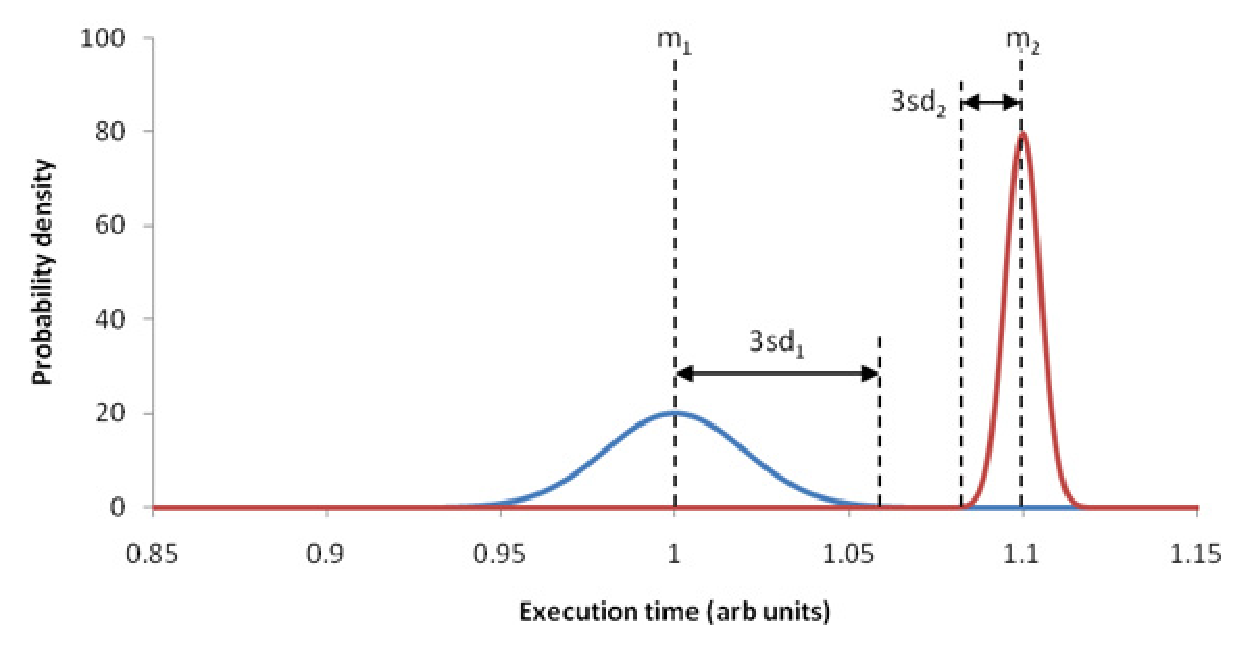
\includegraphics[scale=0.47]{pics/non-overlaping-means}
\label{fig:non-overlapping-means}
}\quad
\subfloat[Overlapping standard deviations.]{%
\centering
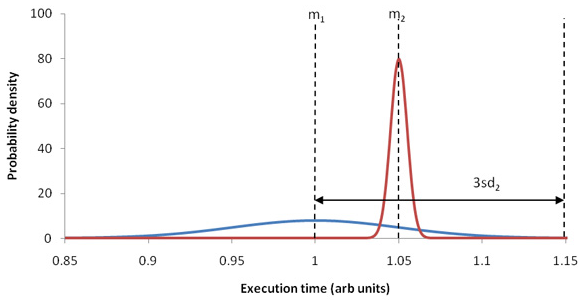
\includegraphics[scale=0.47]{pics/overlaping-means}
\label{fig:overlapping-means}
}}%
\caption{Benchmarks results of two measurements reported with means ($m_i$) and
standard deviations ($sd_i$).}
\end{figure}

% Since the conclusions that we can drawn from the results are based on the mean
% and the standard deviations values, we need to know how much reliability we can
% put into them. Because of all the points that have to be taken care of while
% benchmarking, it is not impossible that some noise still persists while the
% evaluation. With the set of 100 measurements, there are two techniques that can
% inform on the reliability aspect of the statistics, \emph{confidence
% intervals}~\cite{boyer:2008:bench} and the \emph{ANOVA}~\cite{lilja:2000:book} method.
% \begin{description}
% \item[confidence intervals] Means and standard deviations are single computed
% value (i.e. a point estimate), and another run of the benchmark might output
% other results for some reason (e.g. maintenance operations by the system,
% outside of a user control). On the opposite, confidence intervals give a range
% of estimates. A probability p called the confidence level is associated with
% this range. Most commonly, p is chosen to be 95\% and is kept constant during
% confidence interval comparisons. Confidence intervals are intuitive because
% their size indicates reliability: short intervals indicate that the statistic
% is precisely known, while wide intervals indicate uncertainty. For example, if
% the confidence interval for the mean execution of task A is [1, 1.1]
% milliseconds, and that for task B is [0.998, 0.999] milliseconds, then B's
% mean is known with more certainty than A's and is also distinguishably smaller
% (at the same confidence level).
% Confidence intervals can be computed thanks to the
% \emph{bootstrapping}\footnote{Boostrapping:
% \url{http://en.wikipedia.org/wiki/Bootstrapping_(statistics)}} technique, that
% can work for any statistics. A precise explanation of this technique is outside
% the scope of this report.
% \item[ANOVA] Given a set of algorithms to be evaluated, we run them on our
% benchmark and compute for each algorithm a set of 100 measurements. As depicted
% in the Figure~\ref{fig:overlapping-means}, we cannot state with certainty that
% an algorithm A is better than an algorithm B if their interval given by the
% \emph{Vysochansk\"i-Petunin} inequality overlaps. Moreover the difference
% between two algorithms in the other case might not be real if there was some
% noise. \emph{Analysis of the Variance} is a statistical method that tells at
% some confidence degree if one evaluation is statistically better than an other
% one. Thus we can state clearly that an algorithm A is statiscally faster than an
% algorithm B, meaning that the difference observed between the two are real and
% not the consequence of some noise while benchmarking. 
% \end{description}
% ANOVA makes the assumption that measures noises are independent from one
% evaluation to another and that they follow a Gaussian law, while confidence
% intervals does not make any assumptions about the underlaying data.


\chapter{Compression Benchmarks}{
This section describes the benchmark experiments which aim to compare the
various compression methods described previously. The benefits gained with the
use of AFOR algorithms is discussed through two types of data sources. The
first one are unstructured documents: a document is just a bag of words. The
second one are semantically structured documents, e.g. RDF enriched documents.
Since the indexing model for these two types are different, the distribution of
the values within the streams is then also different. Thus the efficiency of a
same compression technique depends on the dataset type.
}
\label{chap:benchmark-cmp}
\section{Benchmarks Settings}
\label{sec:benchmark:framework-cmp}

This section describes the benchmark experiments which aim to compare the
techniques introduced by AFOR with the compression methods described in
Section~\ref{sec:compression:state-of-the-art}. The first experiment measures
the indexing performance based on two aspects:
\begin{inparaenum}[(1)]
\item the indexing time; and 
\item the index size. 
\end{inparaenum}
The indexing time corresponds to the time required to build the index, be it a
traditional inverted index or a node-based inverted index like SIREn. As for
the index size, this time will vary with the compression technique used. The
second experiment compares the query execution performance using indexes built
with different compression techniques.

\paragraph{Data Collection}

In these benchmarks, five datasets were used. Two of them are plain text
datasets which will be used to build traditional inverted indexes, while the
three others are RDF triples and so will be used to build SIREn indexes.

\begin{quotation}
$\Longrightarrow$ Datasets for traditional indexes are composed of:
\begin{description}
\item[Wikipedia:] set of English language Wikipedia articles (~2.5 million
articles). Its total size is 42GB uncompressed.
\item[Blog:] set of 44 million blog posts made between August 1st and October
1st, 2008~\cite{burton:2009:spinn3r}. Its total size is 142GB uncompressed.
\end{description}
\end{quotation}

\begin{quotation}
$\Longrightarrow$ Datasets for the SIREn structure are the following three:
\begin{description}
\item[Geonames:] a geographical database and contains 13.8 million of
entities\footnote{Geonames: \url{http://www.geonames.org/}}. The size is 1.8GB
compressed.
\item[DBPedia:] a semi-structured version of Wikipedia and contains 17.7
million of entities\footnote{DBpedia: \url{http://dbpedia.org/}}. The size is
1.5GB compressed.
\item[Sindice:] a sample of the data collection currently indexed by Sindice.
There is a total of 130.540.675 entities. The size is 6.9GB compressed.
\end{description}
We extracted the entity descriptions from each dataset as pictured in
Figure~\ref{fig:entities}.
\end{quotation}

\section{Indexing Performance}
\label{sec:compression:indexing-performance}

The performance of indexing is compared based on the index size (compression
ratio), commit time (compression speed) and optimise time (compression and
decompression speed). The indexing is performed by adding incrementally 10000
documents at a time and finally by optimising the index.

We report the results of the indexing experiments in
Table~\ref{tab:indexing-performance}. The table comprises two columns with
respect to the indexing time: the total commit time (\emph{Total}) to add all
the documents and the optimisation time (\emph{Opt}). The time collected is
the CPU time used by the current thread and comprises the user time and the
system time. The index size in Table \ref{tab:indexing-performance} is studied
based on the size of each values' streams in the inverted file, and on the total
size of the index. For indexes built with unstructured data (i.e. Wikipedia and
Blog), these streams represent the document identifier, the frequency and the
positions. As for the indexes built on structured data (i.e. DBpedia, Geonames,
Sindice), the streams represent the entity, frequency, attribute, value and
position values. In each tables, the total size is computed by summing the size
of each streams. Bar plots are also provided in order to visualise better the
differences between the techniques.

\paragraph{Commit Time}

Figure~\ref{fig:commit-time} shows the total time spent by each method. As
might be expected, Rice is the slowest method due to its execution flow
complexity on both source type.

On the large unstructured dataset Blog, PFOR is equivalent to Rice in term of
compression speed, since PFOR spends more time in finding the outliers. AFOR-2
and S-64 perform similarly, while AFOR-1 performs as fast as VByte. The drop of
efficiency between AFOR-2 and AFOR-1 is due to the optimization algorithm to
find the best compressing frame. On the small dataset Wikipedia, Rice is
followed by S-64. While FOR, PFOR and VByte perform similarly, AFOR-1 and
AFOR-2 algorithms are the most efficient methods.

On small structured datasets (DBpedia and Geonames), algorithms behave
similarly as described previously. AFOR-3 shows equivalent performance as S-64
on DBpedia, while performing as the best one on Geonames. On a large dataset
(Sindice), VByte is the best-performing method while AFOR-1, AFOR-2, AFOR-3
and S-64 provide a similar commit time. On large datasets (Sindice and Blog),
VByte provides the best commit times, reflecting the benefit from a simple
algorithm.

\begin{figure}
  \centering
    \resizebox{0.8\linewidth}{!}{%
    % \subfloat[Unstructured data]{%
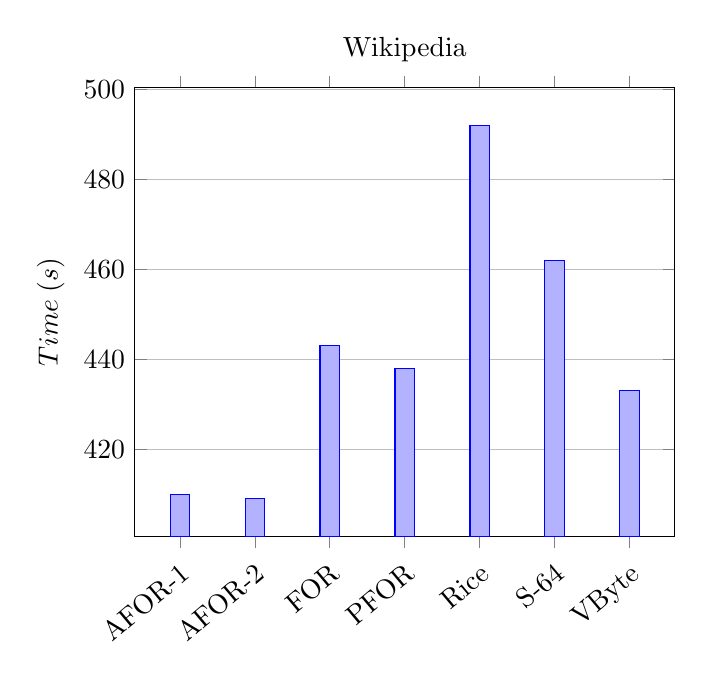
\begin{tikzpicture}[baseline]
\begin{axis}[
ylabel=$Time \; (s)$,
x tick label style={rotate=40, anchor=north east},
xtick={1,...,7},
xticklabels={AFOR-1, AFOR-2, FOR, PFOR, Rice, S-64, VByte},
legend style={at={(0.5,1.13)}, anchor=north, legend columns=-1},
ybar,
ymajorgrids=true,
bar width=7pt,
%enlargelimits=0.015,
title={Wikipedia}
]

\addplot
coordinates {(1, 410) (2, 409) (3, 443) (4, 438) (5, 492) (6, 462) (7, 433)};

\end{axis}
\end{tikzpicture}

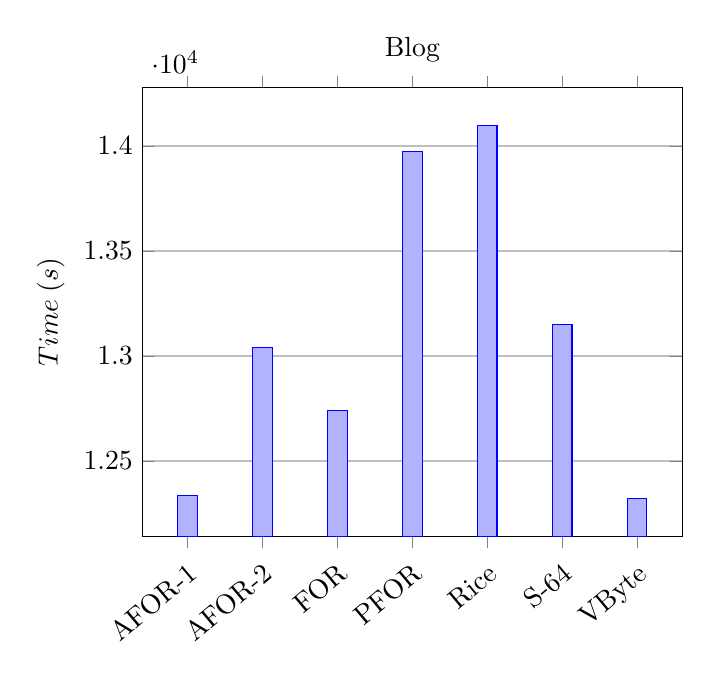
\begin{tikzpicture}[baseline]
\begin{axis}[
ylabel=$Time \; (s)$,
x tick label style={rotate=40, anchor=north east},
xtick={1,...,7},
xticklabels={AFOR-1, AFOR-2, FOR, PFOR, Rice, S-64, VByte},
legend style={at={(0.5,1.13)}, anchor=north, legend columns=-1},
ybar,
ymajorgrids=true,
bar width=7pt,
%enlargelimits=0.015,
title={Blog}
]

\addplot
coordinates {(1, 12337) (2, 13040) (3, 12741) (4, 13972) (5, 14099) (6, 13152) (7, 12320)};

\end{axis}
\end{tikzpicture}
% }
  }
\quad
  \resizebox{\linewidth}{!}{%
    % \subfloat[Structured data]{%
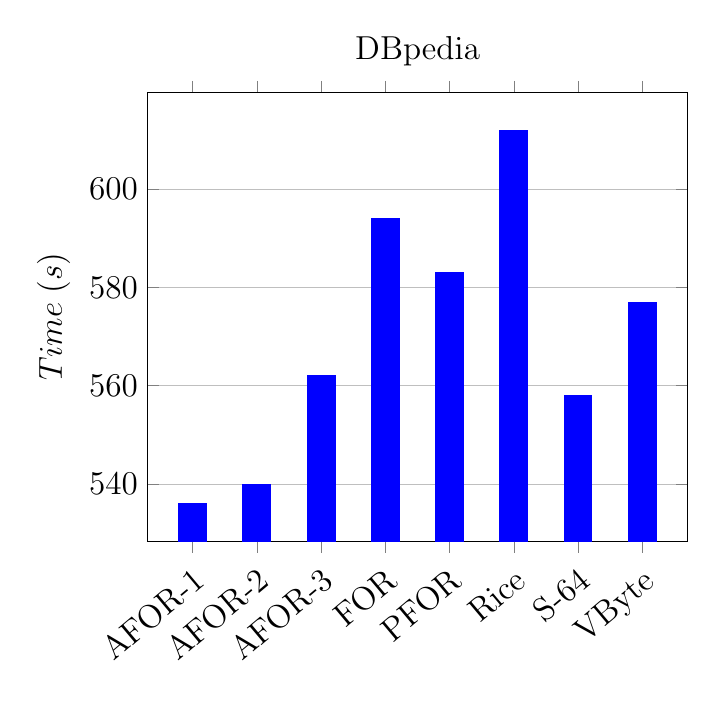
\begin{tikzpicture}[baseline]
\begin{axis}[
ylabel=$Time \; (s)$,
x tick label style={font=\large, rotate=40, anchor=north east},
xtick={1,...,8},
xticklabels={AFOR-1, AFOR-2, AFOR-3, FOR, PFOR, Rice, S-64, VByte},
legend style={at={(0.5,1.13)}, anchor=north, legend columns=-1},
label style={font=\large},
tick label style={font=\large},
title style={font=\large},
ybar,
ymajorgrids=true,
bar width=10pt,
title={DBpedia},
%enlargelimits=0.15,
]
\addplot[draw=blue,fill=blue]
coordinates {(1, 536) (2, 540) (3, 562) (4, 594) (5, 583) (6, 612) (7, 558) (8, 577)};
%\legend{Wikipedia}
\end{axis}
\end{tikzpicture}%
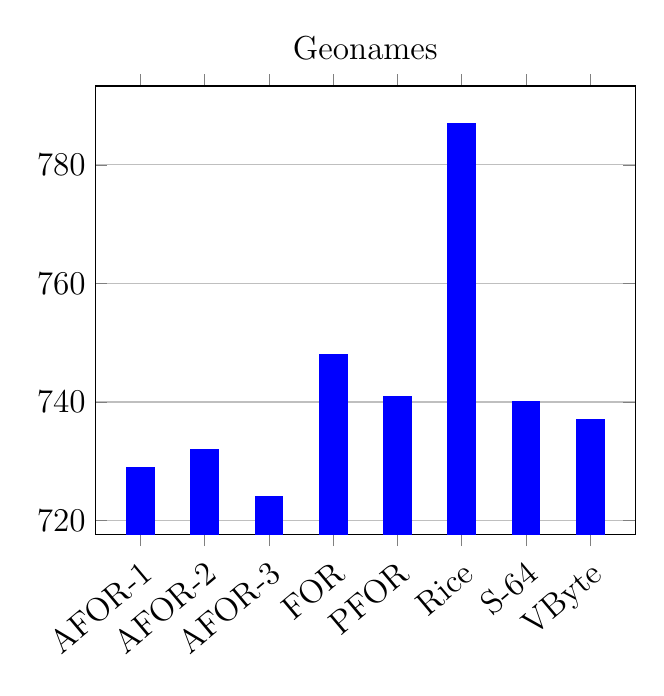
\begin{tikzpicture}[baseline]
\begin{axis}[
x tick label style={font=\large, rotate=40, anchor=north east},
xtick={1,...,8},
xticklabels={AFOR-1, AFOR-2, AFOR-3, FOR, PFOR, Rice, S-64, VByte},
legend style={at={(0.5,1.13)}, anchor=north, legend columns=-1},
label style={font=\large},
tick label style={font=\large},
title style={font=\large},
ybar,
ymajorgrids=true,
bar width=10pt,
title={Geonames},
%enlargelimits=0.15,
]
\addplot[draw=blue,fill=blue]
coordinates {(1, 729) (2, 732) (3, 724) (4, 748) (5, 741) (6, 787) (7, 740) (8, 737)};
%\legend{Blog}
\end{axis}
\end{tikzpicture}
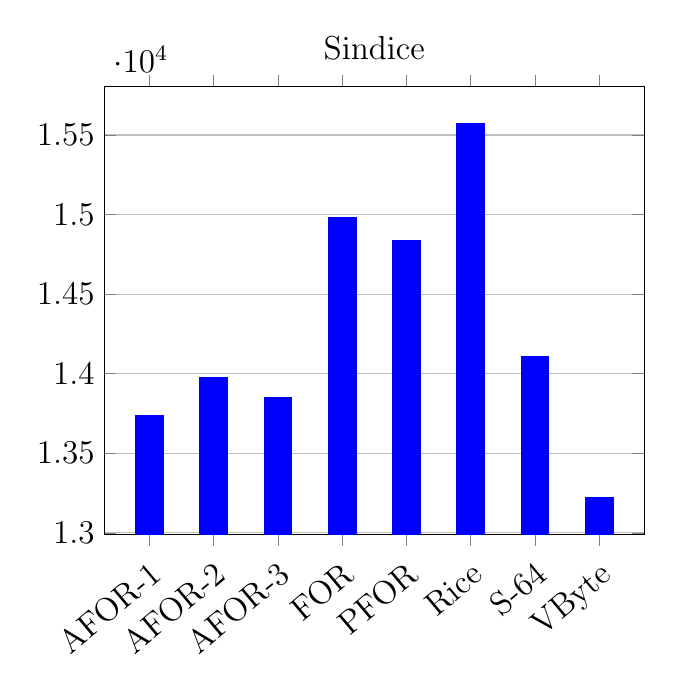
\begin{tikzpicture}[baseline]
\begin{axis}[
x tick label style={font=\large, rotate=40, anchor=north east},
xtick={1,...,8},
xticklabels={AFOR-1, AFOR-2, AFOR-3, FOR, PFOR, Rice, S-64, VByte},
legend style={at={(0.5,1.13)}, anchor=north, legend columns=-1},
label style={font=\large},
tick label style={font=\large},
title style={font=\large},
ybar,
ymajorgrids=true,
bar width=10pt,
title={Sindice},
%enlargelimits=0.15,
]
\addplot[draw=blue,fill=blue]
coordinates {(1, 13734) (2, 13975) (3, 13847) (4, 14978) (5, 14839) (6, 15571) (7, 14107) (8, 13223)};
%\legend{Blog}
\end{axis}
\end{tikzpicture}
% }
  }
	\caption{The total time spent to commit all the batches of 10000 document.}
	\label{fig:commit-time}
\end{figure}

\paragraph{Optimisation Time}

Figure~\ref{fig:optimise-time} shows the optimise time for each methods. The
time to perform the optimisation step is quite different due to the nature of
the operation. The optimisation operation has to read and decompress all the
index segments and compress them back into a single segment. Therefore,
decompression performance is also an important factor, and algorithms having
good decompression speed becomes more competitive.

On both data sources types, while PFOR was similar to Rice in term of commit
time on large datasets (Blog and Sindice), it is ahead of Rice in term of
optimisation time. This can be seen too with FOR on Sindice only. Rice is
penalised by its low decompression speed. The difference introduces by the
decompression performance can also be seen with S-6, which provides performance
close to or even better than VByte. While VByte performs fairly well on
unstructured data, we notice a large overhead on Sindice. The reason is the
distribution of the values on each stream: SIREn produce small values, since
there is a locality effect, i.e. attributes are local to an entity, values are
local to an attribute and positions are local to a value. On traditional
inverted index, position values are local to the whole document, and are then
much bigger. The Table~\ref{tab:indexing-performance} reports a positions
stream of size 20 GBytes at least with every compression techniques, while the
SIREn's streams sizes are bellow 2 GBytes. This difference in compression
ratio produce a large overhead on large datasets (Sindice) with the
decompression speed of VByte.

The best-performing methods are AFOR-1, AFOR-2 and AFOR-3 (structured data
only), with AFOR-3 performing better on large datasets. The AFOR techniques
take the advantage due their optimised compression and decompression routines
and their good compression rate. AFOR-3 is even twice as fast as Rice on the
Sindice dataset.

\begin{figure}
\centering
\begin{minipage}{0.8\linewidth}
  \centering
    \resizebox{0.7\linewidth}{!}{%
    % \subfloat[Unstructured data]{%
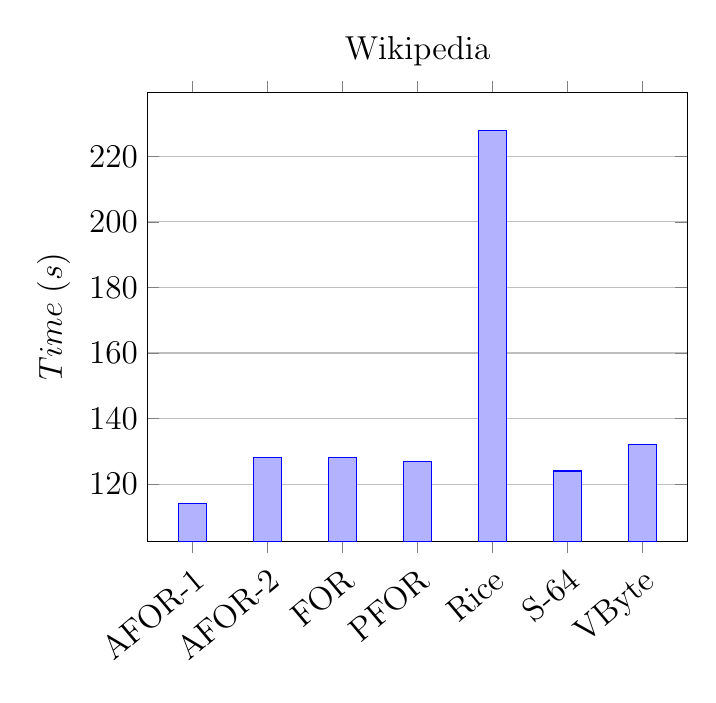
\begin{tikzpicture}[baseline]
\begin{axis}[
ylabel=$Time \; (s)$,
x tick label style={rotate=40, anchor=north east},
xtick={1,...,7},
xticklabels={AFOR-1, AFOR-2, FOR, PFOR, Rice, S-64, VByte},
legend style={at={(0.5,1.13)}, anchor=north, legend columns=-1},
label style={font=\large},
tick label style={font=\large},
title style={font=\large},
ybar,
ymajorgrids=true,
bar width=10pt,
title={Wikipedia},
%enlargelimits=0.15,
]
\addplot
coordinates {(1, 114) (2, 128) (3, 128) (4, 127) (5, 228) (6, 124) (7, 132)};
\end{axis}
\end{tikzpicture}%
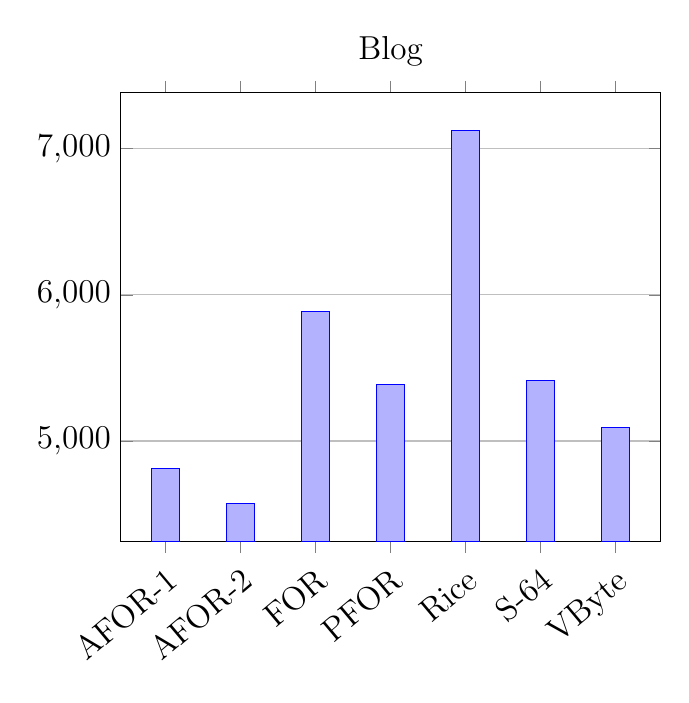
\begin{tikzpicture}[baseline]
\begin{axis}[
x tick label style={rotate=40, anchor=north east},
xtick={1,...,7},
xticklabels={AFOR-1, AFOR-2, FOR, PFOR, Rice, S-64, VByte},
legend style={at={(0.5,1.13)}, anchor=north, legend columns=-1},
label style={font=\large},
tick label style={font=\large},
title style={font=\large},
ybar,
ymajorgrids=true,
bar width=10pt,
title={Blog},
%enlargelimits=0.15,
]
\addplot
coordinates {(1, 4813) (2, 4571) (3, 5888) (4, 5387) (5, 7127) (6, 5414) (7,
5092)};
\end{axis}
\end{tikzpicture}
% }
  }
  \quad
  \resizebox{\linewidth}{!}{%
    % \subfloat[Structured data]{%
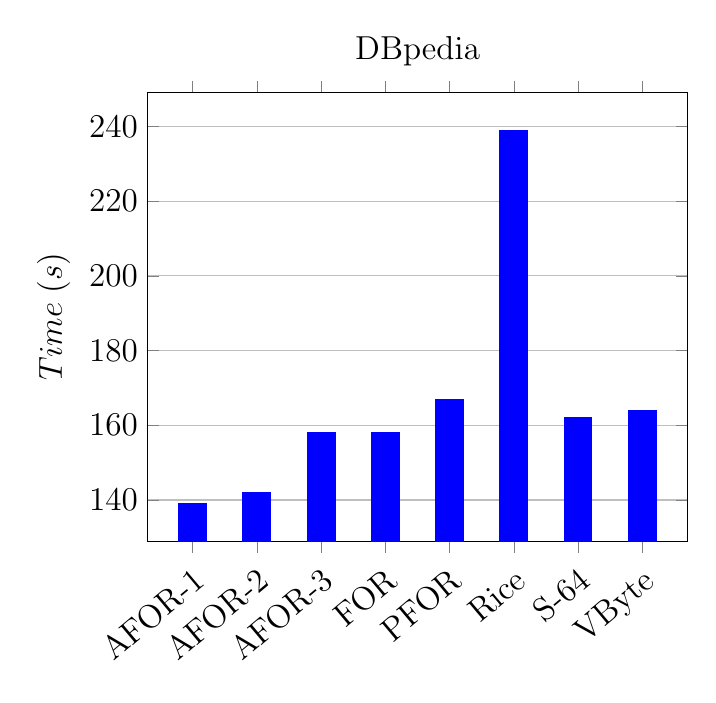
\begin{tikzpicture}[baseline]
\begin{axis}[
ylabel=$Time \; (s)$,
x tick label style={rotate=40, anchor=north east},
xtick={1,...,8},
xticklabels={AFOR-1, AFOR-2, AFOR-3, FOR, PFOR, Rice, S-64, VByte},
legend style={at={(0.5,1.13)}, anchor=north, legend columns=-1},
label style={font=\large},
tick label style={font=\large},
title style={font=\large},
ybar,
ymajorgrids=true,
bar width=10pt,
title={DBpedia},
%enlargelimits=0.15,
]
\addplot[draw=blue,fill=blue]
coordinates {(1, 139) (2, 142) (3, 158) (4, 158) (5, 167) (6, 239) (7, 162) (8, 164)};
\end{axis}
\end{tikzpicture}%
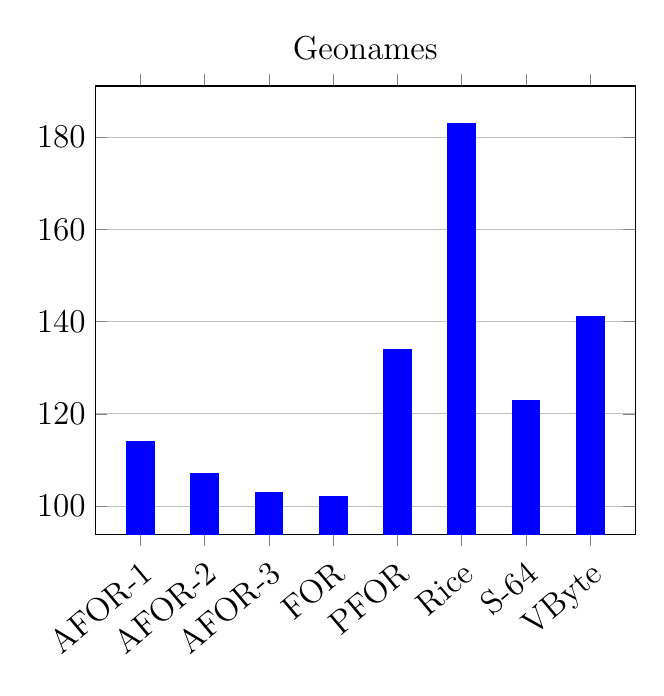
\begin{tikzpicture}[baseline]
\begin{axis}[
x tick label style={rotate=40, anchor=north east},
xtick={1,...,8},
xticklabels={AFOR-1, AFOR-2, AFOR-3, FOR, PFOR, Rice, S-64, VByte},
legend style={at={(0.5,1.13)}, anchor=north, legend columns=-1},
label style={font=\large},
tick label style={font=\large},
title style={font=\large},
ybar,
ymajorgrids=true,
bar width=10pt,
title={Geonames},
%enlargelimits=0.15,
]
\addplot[draw=blue,fill=blue]
coordinates {(1, 114) (2, 107) (3, 103) (4, 102) (5, 134) (6, 183) (7, 123) (8, 141)};
%\legend{Blog}
\end{axis}
\end{tikzpicture}
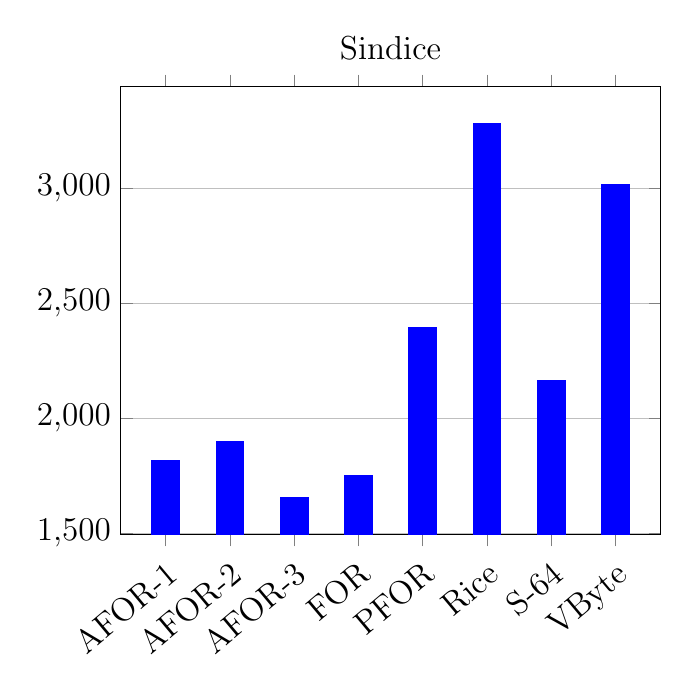
\begin{tikzpicture}[baseline]
\begin{axis}[
x tick label style={rotate=40, anchor=north east},
xtick={1,...,8},
xticklabels={AFOR-1, AFOR-2, AFOR-3, FOR, PFOR, Rice, S-64, VByte},
legend style={at={(0.5,1.13)}, anchor=north, legend columns=-1},
label style={font=\large},
tick label style={font=\large},
title style={font=\large},
ybar,
ymajorgrids=true,
bar width=10pt,
title={Sindice},
%enlargelimits=0.15,
]
\addplot[draw=blue,fill=blue]
coordinates {(1, 1816) (2, 1900) (3, 1656) (4, 1749) (5, 2396) (6, 3281) (7, 2163) (8, 3018)};
%\legend{Blog}
\end{axis}
\end{tikzpicture}
% }
  }
	\caption{The total time spent to optimise the complete index.}
	\label{fig:optimise-time}
\end{minipage}
\end{figure}

\paragraph{Compression Ratio}

Figure~\ref{fig:index-size} shows the total index size achieved by each
method. We can clearly see the inefficiency of the VByte approach. While VByte
performs generally better than FOR on traditional document-centric inverted
indexes like with Wikipedia and Blog datasets, this is not true for inverted
indexes based on a node indexing scheme like SIREn. VByte is not adapted to such
an index due to the properties of the delta-encoded lists of values. Apart
from the entity file, the values are generally very small and the outliers are
rare. In that case, VByte is penalized by its inability to encode a small
integer in less than a byte.

On the contrary, FOR is able to encode many small
integers in one byte. Also, while PFOR is less sensitive to outliers than FOR,
the gain of compression rate provided by PFOR is minimal since outliers are
more rare than in traditional inverted indexes. Indeed we can see that the
distribution of values with a document-centric indexing technique (Wikipedia
and Blog) lead to many outliers, and thus the PFOR algorithm is in that case
efficient.

In contrast, AFOR and S-64 are able to better adapt the encoding to
the value distribution and therefore provide a better compression rate. While
Rice provides the best compression ratio on traditional inverted indexes, AFOR
is able to provide better compression ratio than Rice on the Geonames and
Sindice dataset. Compared to AFOR-2, we can observe in
Table~\ref{tab:indexing-performance} that AFOR-3 provides better compression
rate on the frequency, value and position files, and slightly better on the
entity file. This result corroborates the existence of long runs of 1 in these
files, as explained in Section~\ref{sec:compression:stripping}.

In comparison to normal indexes, Rice provides worse compression ratio than
AFOR on a node indexing scheme index. This can be explained again by the small
values, since Rice does not compress long runs of small values as well as AFOR.

\begin{figure}
\centering
\begin{minipage}{0.8\linewidth}
  \centering
    \resizebox{0.7\linewidth}{!}{%
    % \subfloat[Unstructured data]{%
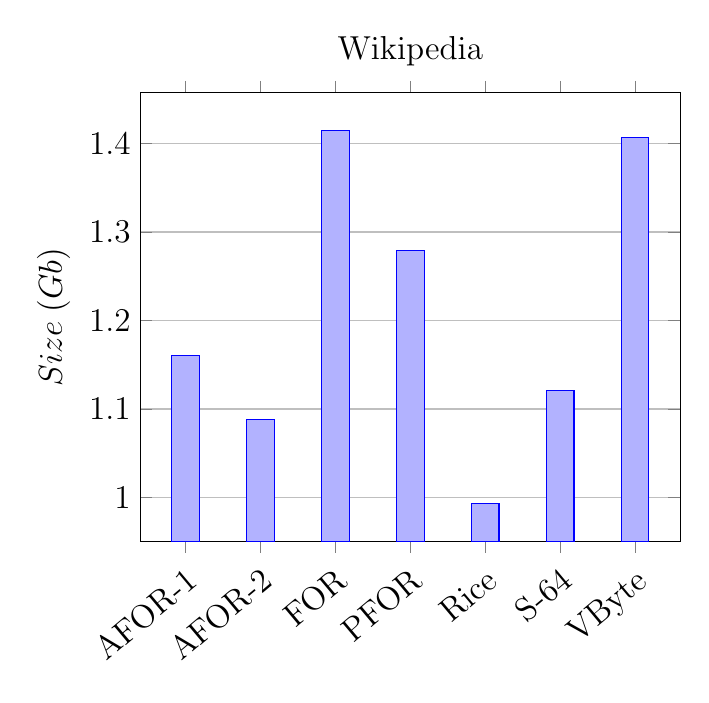
\begin{tikzpicture}[baseline]
\begin{axis}[
ylabel=$Size \; (Gb)$,
x tick label style={rotate=40, anchor=north east},
xtick={1,...,7},
xticklabels={AFOR-1, AFOR-2, FOR, PFOR, Rice, S-64, VByte},
legend style={at={(0.5,1.13)}, anchor=north, legend columns=-1},
label style={font=\large},
tick label style={font=\large},
title style={font=\large},
ybar,
ymajorgrids=true,
bar width=10pt,
title={Wikipedia},
%enlargelimits=0.15,
]
\addplot
coordinates {(1, 1.160) (2, 1.088) (3, 1.415) (4, 1.279) (5, 0.993) (6, 1.121)
(7, 1.407)};
\end{axis}
\end{tikzpicture}%

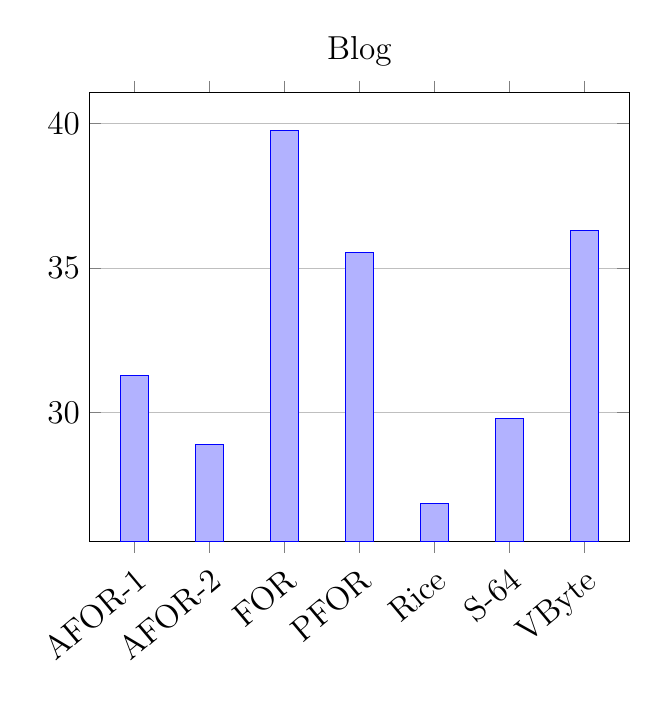
\begin{tikzpicture}[baseline]
\begin{axis}[
x tick label style={rotate=40, anchor=north east},
xtick={1,...,7},
xticklabels={AFOR-1, AFOR-2, FOR, PFOR, Rice, S-64, VByte},
legend style={at={(0.5,1.13)}, anchor=north, legend columns=-1},
label style={font=\large},
tick label style={font=\large},
title style={font=\large},
ybar,
ymajorgrids=true,
bar width=10pt,
title={Blog},
%enlargelimits=0.15,
]
\addplot
coordinates {(1, 31.292) (2, 28.895) (3, 39.777) (4, 35.536) (5, 26.851) (6,
29.800) (7, 36.303)};
\end{axis}
\end{tikzpicture}%
% }
  }
  \quad
  \resizebox{\linewidth}{!}{%
    % \subfloat[Unstructured data]{%
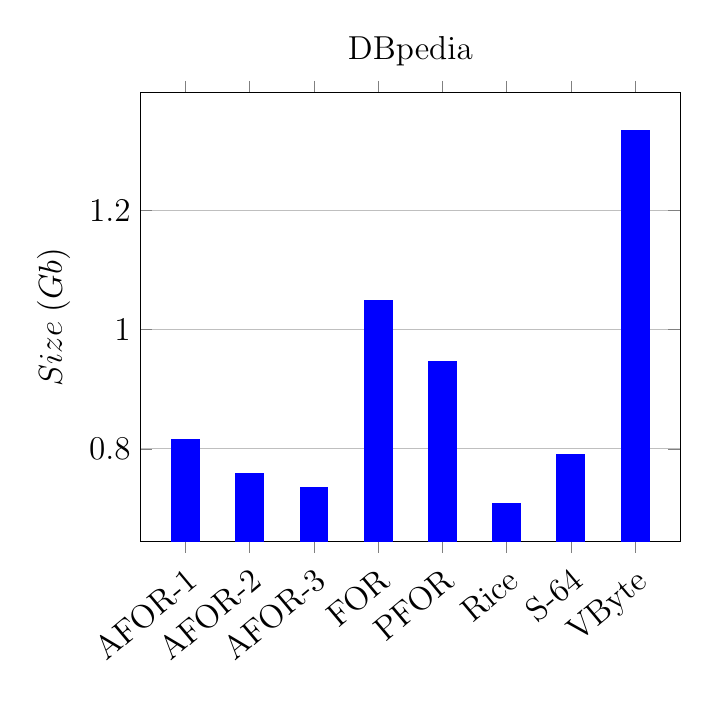
\begin{tikzpicture}[baseline]
\begin{axis}[
ylabel=$Size \; (Gb)$,
x tick label style={rotate=40, anchor=north east},
xtick={1,...,8},
xticklabels={AFOR-1, AFOR-2, AFOR-3, FOR, PFOR, Rice, S-64, VByte},
legend style={at={(0.5,1.13)}, anchor=north, legend columns=-1},
label style={font=\large},
tick label style={font=\large},
title style={font=\large},
ybar,
ymajorgrids=true,
bar width=10pt,
title={DBpedia},
%enlargelimits=0.15,
]
\addplot[draw=blue,fill=blue]
coordinates {(1, 0.816) (2, 0.758) (3, 0.736) (4, 1.049) (5, 0.946) (6, 0.708) (7, 0.791) (8, 1.335)};
\end{axis}
\end{tikzpicture}%
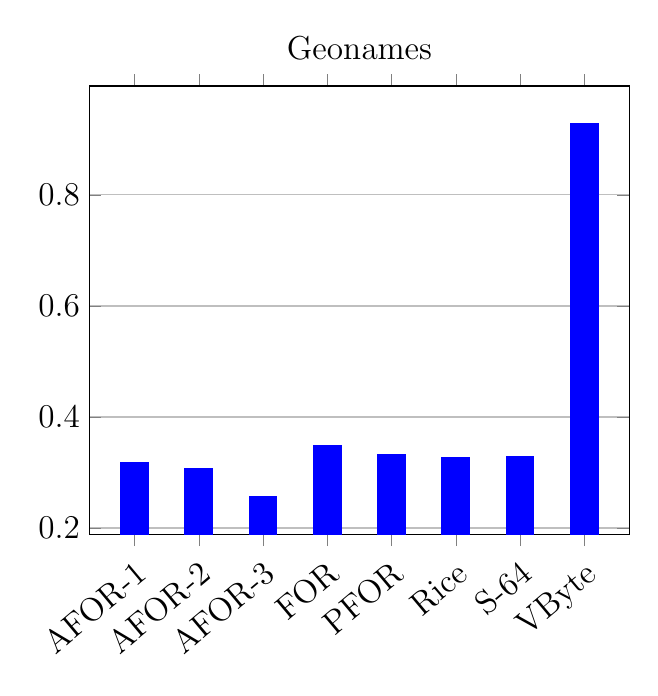
\begin{tikzpicture}[baseline]
\begin{axis}[
x tick label style={rotate=40, anchor=north east},
xtick={1,...,8},
xticklabels={AFOR-1, AFOR-2, AFOR-3, FOR, PFOR, Rice, S-64, VByte},
legend style={at={(0.5,1.13)}, anchor=north, legend columns=-1},
label style={font=\large},
tick label style={font=\large},
title style={font=\large},
ybar,
ymajorgrids=true,
bar width=10pt,
title={Geonames},
%enlargelimits=0.15,
]
\addplot[draw=blue,fill=blue]
coordinates {(1, 0.318) (2, 0.307) (3, 0.256) (4, 0.349) (5, 0.332) (6, 0.327) (7, 0.329) (8, 0.929)};
\end{axis}
\end{tikzpicture}%
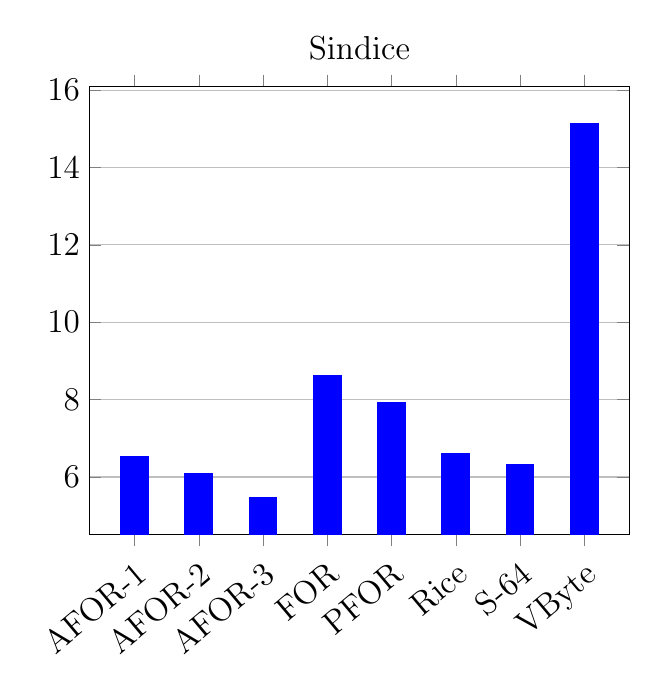
\begin{tikzpicture}[baseline]
\begin{axis}[
x tick label style={rotate=40, anchor=north east},
xtick={1,...,8},
xticklabels={AFOR-1, AFOR-2, AFOR-3, FOR, PFOR, Rice, S-64, VByte},
legend style={at={(0.5,1.13)}, anchor=north, legend columns=-1},
label style={font=\large},
tick label style={font=\large},
title style={font=\large},
ybar,
ymajorgrids=true,
bar width=10pt,
title={Sindice},
%enlargelimits=0.15,
]
\addplot[draw=blue,fill=blue]
coordinates {(1, 6.537) (2, 6.082) (3, 5.475) (4, 8.611) (5, 7.924) (6, 6.605) (7, 6.313) (8, 15.132)};
\end{axis}
\end{tikzpicture}%
% }
  }
	\caption{The index size achieved by each compression technique.}
	\label{fig:index-size}
\end{minipage}
\end{figure}

\paragraph{Conclusion on Indexing Performance}

The indexing experiment shows that the compression speed is also an important
factor to take into consideration when designing a compression algorithm for
an inverted index. Without a good compression speed, the update throughput of
the index is limited. Also the experiment shows that the optimisation
operation is dependent of the decompression performance, and its execution
time can double without a good compression and decompression speed. With
respect to index optimisation, the compression ratio must also be taken into
consideration. While VByte provides in general correct commit times, we can
observe on a large dataset (Sindice) that its performance during optimisation
is limited by its poor compression ratio.

Overall, the method providing the best balance between indexing time, optimise
time and compression ratio is the AFOR family, and this on both structured and
unstructured datasets. AFOR-1 provides fast compression speed and better
compression ratio than FOR and PFOR. AFOR-2 provides a notable additional gain
in compression ratio and optimise time but undergoes a slight increase of
indexing time. AFOR-3 provides another additional gain in compression ratio
while providing better compression speed than AFOR-2.

\section{Querying Performance}
\label{sec:compression:query-performance}

We now compare the decompression performance in real settings, where inverted
indexes are answering queries of various complexities. We report in this
section only the benchmarks done on structured datasets (DBpedia,
Geonames and Sindice), since the performance of query processing on unstructured
datasets is comparable to the ones run on the structured datasets and for
question of clarity also. The raw results are nonetheless reported in the
appendix in the Table~\ref{tab:query-time-TRAD}.

We focus on two main classes of queries, the value and attribute queries, which
are the core elements of a star-shaped query. Among these two classes, we
identify types of keyword queries which represent the common queries received
by a web search engine: conjunction, disjunction and phrase.

\subsection{Query Benchmarking Framework}
\label{sec:bench-query-FW}

In this section we present the types of queries that are run against indexes
compressed with different algorithms.

\subsection{Query Generation}

The queries are generated based on the selectivity of the words composing
them. The word selectivity determines how many entities match a given keyword.
The words are grouped into three selectivity ranges: \emph{high}, \emph{medium}
and \emph{low}. We differentiate also two groups of
words based on their position in the data graph: attribute and value. We
follow the technique described in \cite{errcegovac:2005:vldb} to obtain the
ranges of each word group. We first order the words by their descending
frequency, and then take the first $k$ words whose cumulative frequency is
90\% of all word occurrences as high range. The medium range accounts for the
next 10\%, and the low range is composed of all the remaining words. For the
phrase queries, we follow a similar technique. We first extract all the 2-gram
and 3-gram\footnote{A n-gram is $n$ words that appear contiguously} from the
data collection. We then compute their frequency and sort them by descending
frequency. We finally create the three ranges as explained above. Benchmarks
involving queries with words from low and medium ranges are not reported here
for questions of space, but the performance results are comparable with the
one presented here.

\subsubsection{Value Queries}

Value queries are divided into three types of keyword queries:
\emph{conjunction}, \emph{disjunction} and \emph{phrase} queries. These queries
are restricted to match within one single value, e.g. to find all entities
which have the word ``fantasy'' within a value as in \ref{fig:entities}.
Therefore, the processing of conjunction and disjunction queries relies on the
entity, frequency, attribute and value inverted files. Phrase queries rely on
one additional stream, the position values.

Conjunction and disjunction queries are generated by taking random keywords
from the high range group of words. 2-AND and 2-OR (resp. 4-AND and 4-OR)
denotes conjunction and disjunction queries with 2 random keywords (resp. 4
random keywords). Similarly, a phrase query is generated by taking random
n-grams from the high range group. 2-Phrase (resp. 3-Phrase) denotes phrase
queries with 2-gram (resp. 3-gram). Benchmarks involving queries with words
from low and medium ranges are not reported here for questions of space, but
the performance results are comparable with the ones presented here.

\subsubsection{Attribute Queries}

An attribute query is generated by associating one attribute keyword with one
value query. An attribute keyword is randomly chosen from the high range
groups of attribute words. The associated value query is obtained as explained
previously. An attribute query intersects the result of a value query with an
attribute keyword.

\subsection{Query Benchmark Design}

The benchmarking design used is the one presented in the
Chapter~\ref{chap:benchmarking-framework}. For each type of query, we 
\begin{inparaenum}[(1)]
\item generate a set of 200 random queries which is reused for all the
compression methods, and
\item perform 100 measurements.
\end{inparaenum}
All measurements are made using \emph{warm cache}, i.e., the part of the index
read during query processing is fully loaded in memory.

Query execution time is sensitive to external events which can affect the
final execution time recorded.
% For instance, background system maintenance or
% interruptions as well as cache misses or system exceptions can occur and
% perturb the measurements. All these events are unpredictable and must be
% treated as noise. Therefore, we need to quantify the accuracy of our
% measurements.
% As recommended in \cite{lilja:2000:book}, we report the
% arithmetic mean and the standard deviation of the 100 measurements.
To assess differences between the algorithms, confidence intervals with 95\%
degree of confidence have been used.  The design of the value and attribute
query benchmarks includes three factors:
\begin{description}
\item[Algorithm] having height levels: AFOR-1, AFOR-2, AFOR-3, FOR, PFOR,
Rice, S-64, and VByte;
\item[Query] having six levels: 2-AND, 2-OR, 4-AND, 4-OR, 2-Phrase, and
3-Phrase; and
\item[Dataset] having three levels: DBpedia, Geonames and Sindice. 
\end{description}
Each condition of the design, e.g., AFOR-1 / 2-AND / DBpedia, contains 100
separate measurements.

\subsection{Query Benchmark Results}

We report the results of the query benchmarks in
Table~\ref{tab:value-query-time} and Table~\ref{tab:attribute-query-time} in
the appendix for the value and attribute queries respectively. Based on these
results, we derive multiple graphical charts to better visualise the
differences between each algorithm. These charts are then used to compare and
discuss the performances of each algorithm.

Figure~\ref{fig:avg-value-query-time} and
Figure~\ref{fig:avg-attribute-query-time} report the average query processing
time for the value and attribute queries respectively.
Figure~\ref{fig:avg-value-boolean-query-time} and
Figure~\ref{fig:avg-attribute-boolean-query-time} depict the average
processing time on the Boolean queries.
Figure~\ref{fig:avg-value-phrase-query-time} and
Figure~\ref{fig:avg-attribute-phrase-query-time} depict the average processing
time on the phrase queries (2-Phrase, 3-Phrase). The query processing time are
obtained by summing up the average time of each query from
Table~\ref{tab:value-query-time} for the value queries and
Table~\ref{tab:attribute-query-time} for the attribute queries. For example,
the processing time of AFOR-1 on the DBpedia dataset in
Figure~\ref{fig:avg-value-phrase-query-time} is obtained by summing up the
processing times of the queries 2-Phrase (43.2 ms) and 3-Phrase (32.6 ms)
reported in Table~\ref{tab:value-query-time} in the appendix.

\paragraph{Value Query}

In Figure~\ref{fig:avg-value-query-time}, and in particular on the Sindice
dataset (large dataset), we can distinguish three classes of algorithms: the
techniques based on FOR, a group composed of S-64 and VByte, and finally Rice.
The FOR group achieves relatively similar results, with AFOR-2 slightly behind
the others.

Rice has the worst performance for every query and dataset, followed by VByte.
Nonetheless Rice performs in many cases twice as slow as VByte. In
Figure~\ref{fig:avg-value-boolean-query-time}, S-64 provides similar
performance to VByte on Boolean queries but we can see in
Figure~\ref{fig:avg-value-phrase-query-time} that it is faster than VByte on
phrase queries. However, S-64 stays behind FOR, PFOR and AFOR in all the cases.

FOR, PFOR and AFOR have relatively similar performances on all the Boolean
queries and all the datasets. PFOR seems to provide generally slightly better
performance on the phrase queries but seems to be slower on Boolean queries.

\begin{figure}
  \centering
  \subfloat[Boolean Query]{%
    \resizebox{0.45\linewidth}{!}{%
      
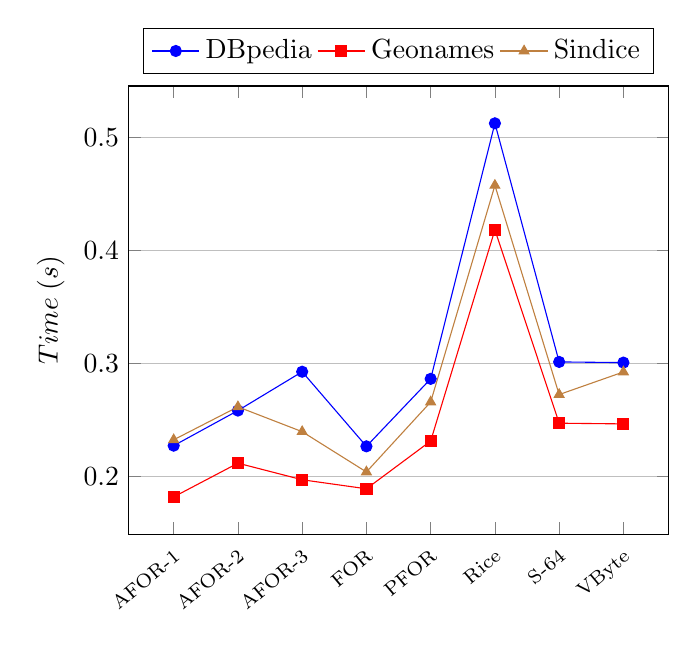
\begin{tikzpicture}
\begin{axis}[
ylabel=$Time \; (s)$,
x tick label style={font=\scriptsize, rotate=40, anchor=north east},
xtick={1,...,8},
xticklabels={AFOR-1, AFOR-2, AFOR-3, FOR, PFOR, Rice, S-64, VByte},
legend style={at={(0.5,1.13)}, anchor=north, legend columns=-1},
%ybar,
ymajorgrids=true,
%bar width=5pt,
]

\addplot[blue,mark=*]
coordinates {(1, 0.2271) (2, 0.2582) (3, 0.2926) (4, 0.2265) (5, 0.2863) (6, 0.5127) (7, 0.3013) (8, 0.3007)};
\addplot[red,mark=square*]
coordinates {(1, 0.1817) (2, 0.2116) (3, 0.1969) (4, 0.1889) (5, 0.2312) (6, 0.4184) (7, 0.2470) (8, 0.2464)};
\addplot[brown,mark=triangle*]
coordinates {(1, 0.2323) (2, 0.2615) (3, 0.2395) (4, 0.2038) (5, 0.2658) (6, 0.4577) (7, 0.2724) (8, 0.2924)};

\legend{DBpedia, Geonames, Sindice}

\end{axis}
\end{tikzpicture}%

  	}
  	\label{fig:avg-value-boolean-query-time}
  }\quad%
  \subfloat[Phrase Query]{%
    \resizebox{0.45\linewidth}{!}{%
      
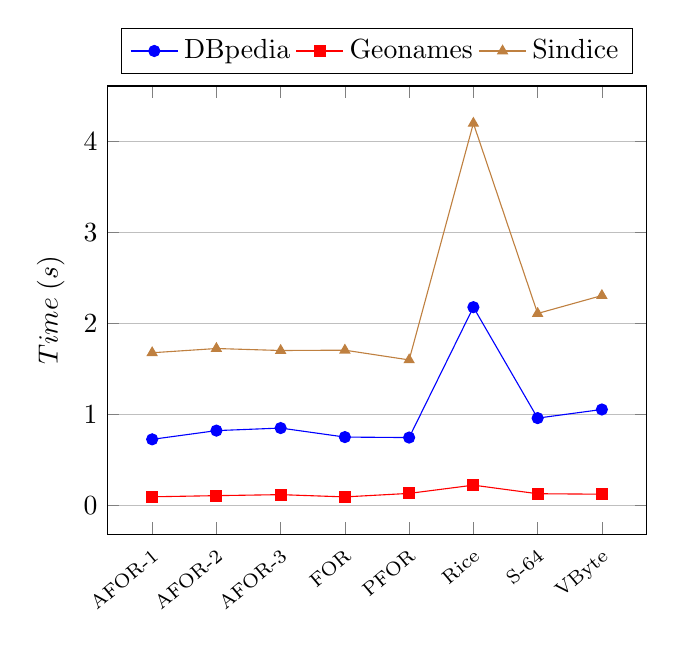
\begin{tikzpicture}
\begin{axis}[
ylabel=$Time \; (s)$,
x tick label style={font=\scriptsize, rotate=40, anchor=north east},
xtick={1,...,8},
xticklabels={AFOR-1, AFOR-2, AFOR-3, FOR, PFOR, Rice, S-64, VByte},
legend style={at={(0.5,1.13)}, anchor=north, legend columns=-1},
%ybar,
ymajorgrids=true,
%bar width=5pt,
]

\addplot[blue,mark=*]
coordinates {(1, 0.7267) (2, 0.8225) (3, 0.8506) (4, 0.7516) (5, 0.7462) (6, 2.1778) (7, 0.9598) (8, 1.0544) };
\addplot[red,mark=square*]
coordinates {(1, 0.0959) (2, 0.1085) (3, 0.1196) (4, 0.0947) (5, 0.1333) (6, 0.2237) (7, 0.1296) (8, 0.1245)};
\addplot[brown,mark=triangle*]
coordinates {(1, 1.6773) (2, 1.7239) (3, 1.702) (4, 1.7056) (5, 1.5986) (6, 4.1963) (7, 2.1086) (8, 2.3053)};

\legend{DBpedia, Geonames, Sindice}

\end{axis}
\end{tikzpicture}%

    }
    \label{fig:avg-value-phrase-query-time}
  }%
	\caption{The average processing time for the value queries that is achieved
	by each compression technique.}
	\label{fig:avg-value-query-time}
\end{figure}

\paragraph{Attribute Query}

In Figure~\ref{fig:avg-attribute-query-time}, and in particular on Sindice, we
can again distinguish the same three classes of algorithms. However, the
performance gap between S-64 and VByte becomes wider.

Rice has again the worst performance for every query and dataset. Compared to
the performance on value queries, we can see in
Figure~\ref{fig:avg-attribute-boolean-query-time} that S-64 provides similar
performance to PFOR and AFOR-2 on Boolean queries. FOR and AFOR-3 seem to be
the best performing methods on Boolean queries. With respect to the phrase
queries in Figure~\ref{fig:avg-attribute-phrase-query-time}, S-64 has better
performance than VByte. However, PFOR does not achieve any more the best
performance on phrase queries. Instead, it seems that AFOR-2 and FOR achieve a
slightly better processing time.

FOR, PFOR and AFOR have again relatively similar performances on all the
queries and all the datasets. AFOR-2 appears to be slower to some degree,
while the gap between AFOR-3 and PFOR becomes less perceptible.

\begin{figure}
  \centering
  \subfloat[Boolean Query]{%
    \resizebox{0.45\linewidth}{!}{%
      
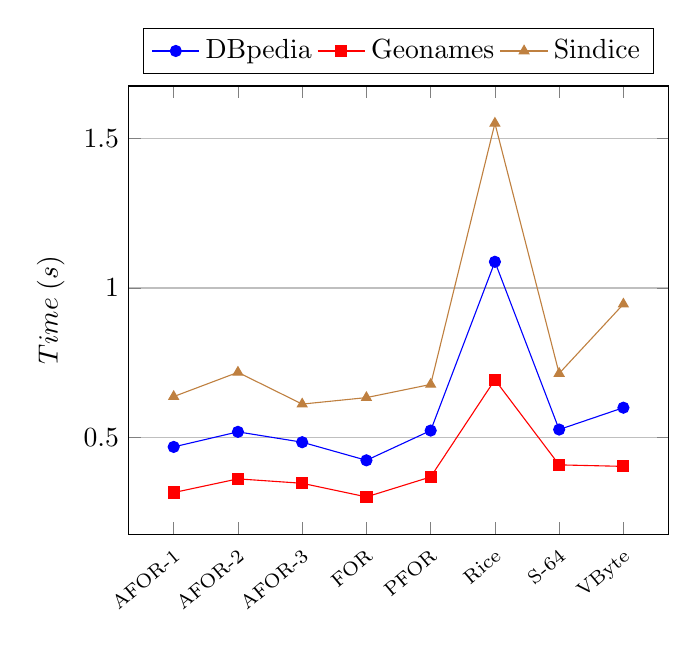
\begin{tikzpicture}
\begin{axis}[
ylabel=$Time \; (s)$,
x tick label style={font=\scriptsize, rotate=40, anchor=north east},
xtick={1,...,8},
xticklabels={AFOR-1, AFOR-2, AFOR-3, FOR, PFOR, Rice, S-64, VByte},
legend style={at={(0.5,1.13)}, anchor=north, legend columns=-1},
%ybar,
ymajorgrids=true,
%bar width=7pt,
]

\addplot[blue,mark=*]
coordinates {(1, 0.4692) (2, 0.5195) (3, 0.4849) (4, 0.4244) (5, 0.5238) (6, 1.0875) (7, 0.5272) (8, 0.6002)};
\addplot[red,mark=square*]
coordinates {(1, 0.3167) (2, 0.3625) (3, 0.3477) (4, 0.3022) (5, 0.3689) (6, 0.6936) (7, 0.4092) (8, 0.4042)};
\addplot[brown,mark=triangle*]
coordinates {(1, 0.6373) (2, 0.7183) (3, 0.6122) (4, 0.6339) (5, 0.6779) (6, 1.55) (7, 0.7146) (8, 0.946)};

\legend{DBpedia, Geonames, Sindice}

\end{axis}
\end{tikzpicture}


  	}
  	\label{fig:avg-attribute-boolean-query-time}
  }\quad%
  \subfloat[Phrase Query]{%
    \resizebox{0.45\linewidth}{!}{%
      
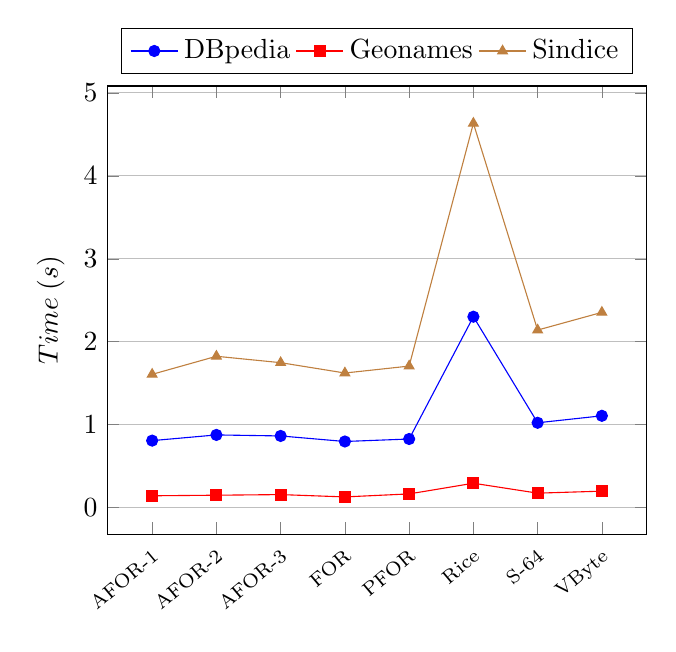
\begin{tikzpicture}
\begin{axis}[
ylabel=$Time \; (s)$,
x tick label style={font=\scriptsize, rotate=40, anchor=north east},
xtick={1,...,8},
xticklabels={AFOR-1, AFOR-2, AFOR-3, FOR, PFOR, Rice, S-64, VByte},
legend style={at={(0.5,1.13)}, anchor=north, legend columns=-1},
%ybar,
ymajorgrids=true,
%bar width=7pt,
]

\addplot[blue,mark=*]
coordinates {(1, 0.8081) (2, 0.8767) (3, 0.8644) (4, 0.7976) (5, 0.8275) (6, 2.302) (7, 1.0232) (8, 1.1072)};
\addplot[red,mark=square*]
coordinates {(1, 0.143) (2, 0.1499) (3, 0.1574) (4, 0.1293) (5, 0.1656) (6, 0.2943) (7, 0.1747) (8, 0.1988)};
\addplot[brown,mark=triangle*]
coordinates {(1, 1.6073) (2, 1.825) (3, 1.7478) (4, 1.6231) (5, 1.7067) (6, 4.6336) (7, 2.1409) (8, 2.3544)};

\legend{DBpedia, Geonames, Sindice}

\end{axis}
\end{tikzpicture}


    }
    \label{fig:avg-attribute-phrase-query-time}
  }%
	\caption{The average processing time for the attribute queries that is
	achieved by each compression technique.}
	\label{fig:avg-attribute-query-time}
\end{figure}

\section{Performance Trade-Off}

We report in Figure~\ref{fig:trade-off-time-bytes} the trade-off between the
total query processing time and the compression ratio among all the techniques
on the Sindice dataset. The total query time has been obtained by summing up
the average time of all the queries. The compression ratio is based on the
number of bytes read during query processing which are reported in
Table~\ref{tab:value-query-time} and Table~\ref{tab:attribute-query-time} in
the appendix.
We can distinctively see that the AFOR techniques are close to Rice in term of
compression ratio, while being relatively close to FOR and PFOR in term of
query processing time. Compared to AFOR-1, AFOR-2 achieves a better
compression rate in exchange of a slightly slower processing time. However,
AFOR-3 accomplishes a better compression rate with a processing time close to
AFOR-1.

\begin{figure}
  \centering
  \subfloat[Value Query]{%
    \resizebox{0.47\linewidth}{!}{%
      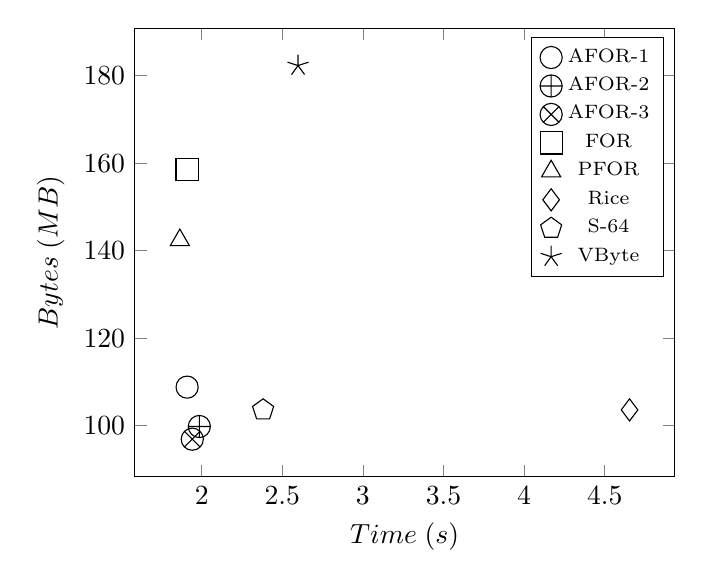
\begin{tikzpicture}
\begin{axis}[
scatter/classes={
	a={mark=o},
	b={mark=oplus},
	c={mark=otimes},
	d={mark=square},
	e={mark=triangle},
	f={mark=diamond},
	g={mark=pentagon},
	h={mark=star}
  },
  ylabel=$Bytes \; (MB)$,
  xlabel=$Time \; (s)$,
  mark options={scale=2},
  legend style={font=\scriptsize}
]

\addplot[scatter, only marks]
plot[scatter src=explicit symbolic]
coordinates {
(1.9096, 108.8) [a]
(1.9854, 99.8) [b]
(1.9415, 96.9) [c]
(1.9094, 158.5) [d]
(1.8644, 142.4) [e]
(4.654, 103.6) [f]
(2.381, 103.6) [g]
(2.5977, 182.3) [h]
};

\legend{AFOR-1, AFOR-2, AFOR-3, FOR, PFOR, Rice, S-64, VByte}

\end{axis}
\end{tikzpicture}
  	}
  }%
  \subfloat[Attribute Query]{%
    \resizebox{0.47\linewidth}{!}{%
      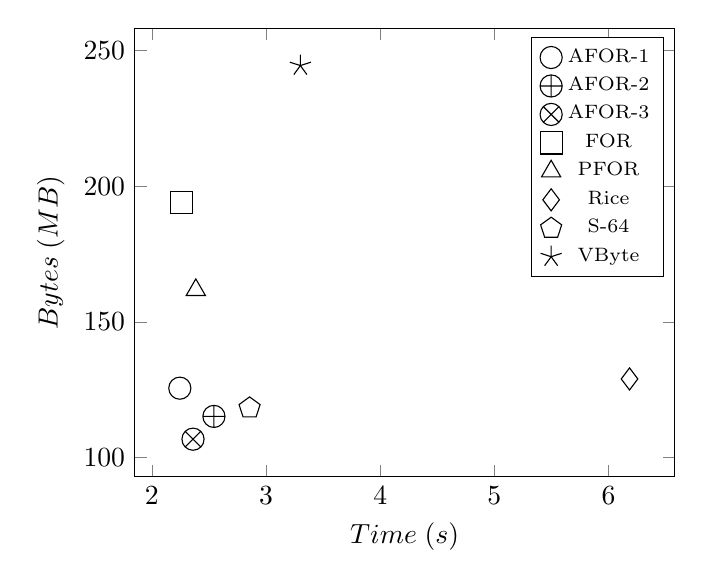
\begin{tikzpicture}
\begin{axis}[
	scatter/classes={
	a={mark=o},
	b={mark=oplus},
	c={mark=otimes},
	d={mark=square},
	e={mark=triangle},
	f={mark=diamond},
	g={mark=pentagon},
	h={mark=star}
  },
  ylabel=$Bytes \; (MB)$,
  xlabel=$Time \; (s)$,
  mark options={scale=2},
  legend style={font=\scriptsize},
]

\addplot[only marks]
plot[scatter, scatter src=explicit symbolic]
coordinates {
 (2.2446, 125.6) [a]
 (2.5433, 115.2) [b]
 (2.36, 106.8) [c]
 (2.257, 194.0) [d]
 (2.3846, 161.8) [e]
 (6.1836, 129.0) [f]
 (2.8555, 118.3) [g]
 (3.3004, 244.5) [h]
};
\legend{AFOR-1, AFOR-2, AFOR-3, FOR, PFOR, Rice, S-64, VByte}
\end{axis}
\end{tikzpicture}
    }
  }%
	\caption{A graphical comparison showing the trade-off between querying time
	and compression ratio on the Sindice dataset. The compression ratio is
	represented by the number of bytes read during the query processing.}
	\label{fig:trade-off-time-bytes}
\end{figure}

We report in Figure~\ref{fig:trade-off-query-update} the trade-off between the
total query processing time and the indexing time among all the techniques on
the Sindice dataset. The indexing time has been obtained by summing up the
commit and optimise time from Table~\ref{tab:indexing-performance} of the
appendix. We can distinctively see that the AFOR techniques achieve the best
trade-off between indexing and querying time. AFOR-3 produce very similar
indexing and querying times to AFOR-1, while providing a much better
compression rate. It is interesting to notice that PFOR provides a slightly
better querying time than FOR but at the price of a much slower compression.
Also, S-64 and VByte provide a relatively close performance trade-off. To
conclude, AFOR-3 seems to offer the best compromise between querying time,
indexing time, and compression rate.

\begin{figure}
  \centering
  \subfloat[Value Query]{%
    \resizebox{0.47\linewidth}{!}{%
      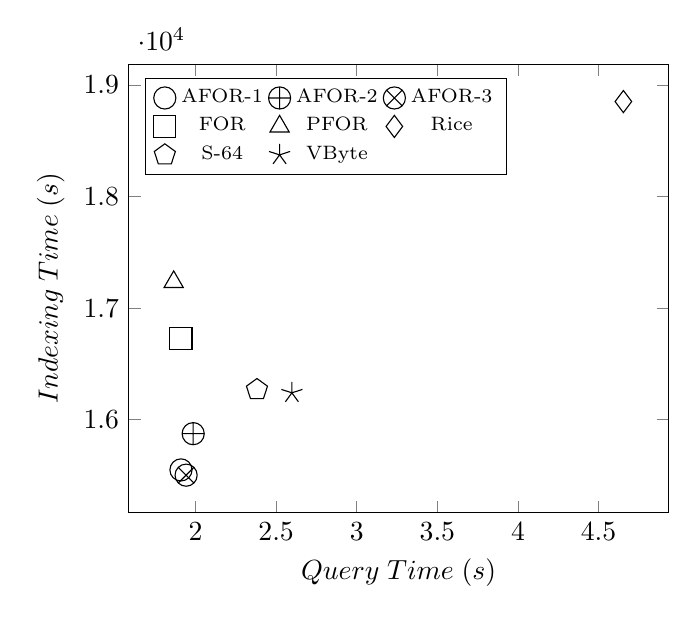
\begin{tikzpicture}
\begin{axis}[%
  scatter/classes={%
	a={mark=o},%
	b={mark=oplus},%
	c={mark=otimes},%
	d={mark=square},%
	e={mark=triangle},%
	f={mark=diamond},%
	g={mark=pentagon},%
	h={mark=star}
  },
  ylabel=$Indexing \; Time \; (s)$,
  xlabel=$Query \; Time \; (s)$,
  mark options={scale=2},
  legend columns=3,
  legend pos=north west,
  legend style={font=\scriptsize, anchor=north west, legend columns=3},
]

\addplot[only marks]
plot[scatter,scatter src=explicit symbolic]
coordinates {%
(1.9096, 15550) [a]
(1.9854, 15875) [b]
(1.9415, 15503) [c]
(1.9094, 16727) [d]
(1.8644, 17235) [e]
(4.654, 18852) [f]
(2.381, 16270) [g]
(2.5977, 16241) [h]
};%
\legend{AFOR-1, AFOR-2, AFOR-3, FOR, PFOR, Rice, S-64, VByte}
\end{axis}
\end{tikzpicture}
  	}
  }%
  \subfloat[Attribute Query]{%
    \resizebox{0.47\linewidth}{!}{%
      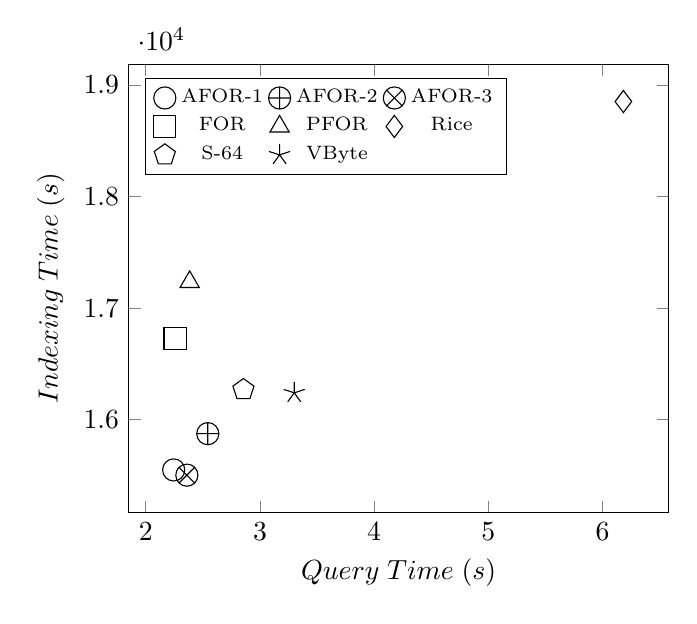
\begin{tikzpicture}
\begin{axis}[
  scatter/classes={
	a={mark=o},%
	b={mark=oplus},%
	c={mark=otimes},%
	d={mark=square},%
	e={mark=triangle},%
	f={mark=diamond},%
	g={mark=pentagon},%
	h={mark=star}
  },
  ylabel=$Indexing \; Time \; (s)$,
  xlabel=$Query \; Time \; (s)$,
  mark options={scale=2},
  legend columns=3,
  legend pos=north west,
  legend style={font=\scriptsize, anchor=north west, legend columns=3}
]

\addplot[only marks]
plot[scatter,mark=*,scatter src=explicit symbolic]
coordinates {
(2.2446, 15550) [a]
(2.5433, 15875) [b]
(2.3600, 15503) [c]
(2.2570, 16727) [d]
(2.3846, 17235) [e]
(6.1836, 18852) [f]
(2.8555, 16270) [g]
(3.3004, 16241) [h]
};
\legend{AFOR-1, AFOR-2, AFOR-3, FOR, PFOR, Rice, S-64, VByte}
\end{axis}
\end{tikzpicture}
    }
  }%
\caption{A graphical comparison of the compression techniques showing the
trade-off between querying time and indexing time on the Sindice dataset.}
\label{fig:trade-off-query-update}
\end{figure}

\section{Discussion}

In general, even if FOR has more data to read and decompress, it still
provides one of the best query execution time. The reason is that our
experiments are performed using warm cache. We therefore ignore the cost of
disk IO accesses and measure exclusively the decompression efficiency of the
methods. With a cold cache, i.e., when IO disk accesses have to be performed,
we expect a drop of performance for algorithms with a low compression ratio
such as FOR and PFOR compared to AFOR-2 and AFOR-3.

Compression and decompression performance do not only depend on the
compression ratio, but also on the execution flow of the algorithm and on the
number of cycles needed to compress or decompress an integer. Therefore,
CPU-optimised algorithms which provides at the same time a good compression
ratio are most likely to increase the update and query throughput of web
search engines. In that context, AFOR seems to be a good candidate since it is
well balanced in all aspects: it provides very good indexing and querying
performance and one of the best compression ratio.

The Simple encoding family is somehow similar to AFOR. At each iteration, S-64
encodes or decodes a variable number of integers using CPU optimised routines.
AFOR is however not tied to the size of a machine word, and is thus simpler to
implement and provides better compression ratio, compression speed and
decompression speed.


\chapter{Scalability of SIREn}{
In the previous experiments, we have seen that AFOR-3 is the most suitable
compression technique for an entity inverted index like SIREn. Based on these
results, we perform a stress test of the entity index compressed with AFOR-3
through a large scale experiment which simulates the conditions of a real Web
Data search engine such as Sindice. We use the full Sindice data collection to
create three indexes of increasing size and we generate a set of star queries
of increasing complexity. We compare the query rate (queries per second)
the system can answer with respect to the size of the index and the complexity
of the query.
}
\label{chap:scalability}
\section{Benchmarking Framework}

In this section we discuss the ability of the AFOR compression techniques
family to scale with the growing size of the compressed data.

\paragraph{Data Collection}

The full Sindice data collection is currently composed of more
than 120 millions of documents among 90.000 datasets. For each dataset, we
extracted the entities as depicted in Figure~\ref{fig:entities}.
We filtered out all the entity descriptions containing less than two values.
After filtering, there is a total of 907.542.436 entities for 4.689.599.183
RDF triples. We create three datasets: \emph{Small} containing 226.129.319
entities for 1.240.674.545 RDF triples; \emph{Medium} containing
447.305.647 entities for 2.535.658.099 RDF triples; and \emph{Large}
containing the complete collection of entities.

\paragraph{Query Benchmark Design}

We generate star queries of increasing complexity, starting with 1 attribute
query up to 16. Using an uniform distribution for the random method, each
attribute query is generated by selecting at random an attribute term from the
high, medium or low selectivity ranges. The associated value query is generated
by selecting at random a conjunction (2-AND or 4-AND) or a disjunction (2-OR or
4-OR). Each term of the value query is selected from the high, medium or low
selectivity ranges at random. Such a query generation scheme provides star
queries of average complexity, i.e. queries composed of terms from any
selectivity range.

With respect to the creation of the three selectivity ranges for the value
terms, we observed the presence of a longer tail in the term frequency
distribution compared to the previous experiments. Consequently, we modified
the way the ranges are computed. The high range represents the first $k$ words
whose cumulative frequency is 50\% of all word occurrences. The medium range
accounts for the next 30\%, and the low range is composed of all the remaining
words.

Following the benchmark design in Chapter~\ref{chap:benchmarking-framework}, for
each type of star query, we \begin{inparaenum}[(1)]
\item generate a set of 400 random queries, and 
\item perform 100 measurements.
\end{inparaenum}
Each measurement is made using \emph{warm cache}. A measurement records the
query rate, i.e. the number of query the system can process per second, using
a single thread.

The design of the scalability benchmark includes three factors:
\begin{description}
\item[Dataset] having three levels: Small, Medium and Large. 
\item[Query Size] having five levels: 1, 2, 4, 8, and 16.
\item[Term Selectivity] having two levels: Low-Medium-High (LMH) and
Medium-High (MH).
\end{description}
Each condition of the design, e.g., Small / 4 / LMH, contains 100 separate
measurements. The term selectivity denotes the selectivity ranges that has
been used to generate the query terms. For example, the MH selectivity level
means that all the query terms have been generated from either the medium or
high range.
 
\section{Indexing Performance}

We report that during the indexing of the data collection per batch of 100.000
entities, the commit time stayed constant, with an average commit time of 2062
milliseconds. The optimisation of the full index were performed in 119
minutes. The size of the five inverted files is 19.279 GB, with 10.912 GB for
the entity file, 0.684 GB for the frequency file, 3.484 GB for the attribute
file, 1.810 GB for the value file and 2.389 GB for the position file. The size
of the dictionary is 8.808 GB and the size of the skip lists, i.e., the data
structure for self-indexing further presented in
Chapter~\ref{sec:self-indexing}, is 7.644 GB. The total size of the index is
35.731 GB which represents an average of 8 bytes per RDF statement (i.e.
triple).

\section{Querying Performance}
\label{sec:scalability:query}

We report the results of the scalability benchmark in
Table~\ref{tab:scalability:query-rate} of the appendix. Based on these results,
we derive two graphical charts in Figure~\ref{fig:query-rate} to better
visualise the evolution of the query rate with respect to the size of the
dataset and the complexity of the queries.

With respect to the size of the queries, we can observe that the query rate
increases with the number of attribute value pairs until a certain point (up
to 2 or 4 pairs), and then starts to decrease. The lowest query rate is
obtained when the star query is composed of only one attribute query. Such a
query produces a higher number of hits compared to other queries, and as a
consequence the system has to read more data. On the contrary, the precision
of the query increases with the number of attribute queries, and the chance of
having a large number of hits decreases consequently.
% In that case, the
% self-indexing technique provides considerable benefits since it enables the
% system to avoid a large amount of unnecessary record comparisons and to answer
% complex queries in sub-linear time.

Concerning the term selectivity, we can note a drop of query rate between
Figure~\ref{fig:low-query-rate} where query terms of low selectivity are
employed and Figure~\ref{fig:medium-query-rate} where query terms of low
selectivity is not employed. In the later case, the system has to perform more
record comparisons.
% Whenever a term with a low selectivity is used in the
% query, the system is able to take advantage of the self-indexing and to skip a
% larger number of records during query processing.

The size of the data collection has only a limited impact on the query rate.
The reason is that the query processing complexity is bound by the size of the
inverted lists which is itself dependent of the term distribution. Therefore,
the size of the data collection has a weak influence on the size of the
inverted lists, apart for very frequent terms. A term with a low or medium
selectivity will have a short inverted lists even if the data collection is
very large.

To conclude, the results show that the query rate of the system scales
gracefully with the size of the data and the complexity of the query. A
single-threaded system is able to sustain a query rate of 17 queries per
second up to 292 queries per second depending of the kind of queries. At this
rate, the system is able to support many requests, or users, at the same time.

\begin{figure}
  \centering
  \subfloat[Query rate with LMH selectivity]{%
    \resizebox{0.45\linewidth}{!}{%
      
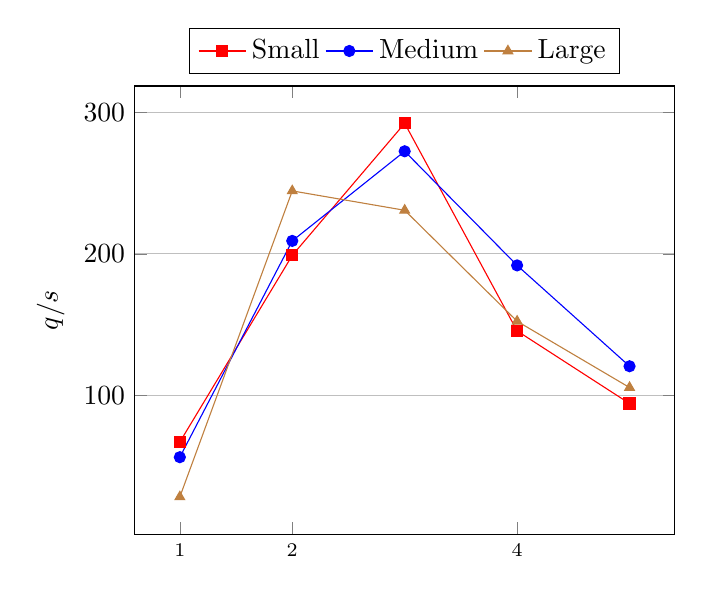
\begin{tikzpicture}
\begin{axis}[
ylabel=$q/s$,
x tick label style={font=\scriptsize},
legend style={at={(0.5,1.13)}, anchor=north, legend columns=-1},
xtick={1,2,4,8,16},
%ybar,
ymajorgrids=true,
%bar width=5pt,
]

\addplot[red,mark=square*]
coordinates {(1, 66.884) (2, 198.906) (3, 292.334) (4, 145.492) (5, 94.124)};
\addplot[blue,mark=*]
%coordinates {(1, 56.163) (2, 209.161) (3, 272.554) (4, 31.234) (5, 120.493)};
coordinates {(1, 56.163) (2, 209.161) (3, 272.554) (4, 191.828) (5, 120.493)};
\addplot[brown,mark=triangle*]
coordinates {(1, 28.062) (2, 244.529) (3, 230.814) (4, 152.311) (5, 105.441)};

\legend{Small, Medium, Large}

\end{axis}
\end{tikzpicture}%

  	}
  	\label{fig:low-query-rate}
  }\quad%
  \subfloat[Query rate with MH selectivity]{%
    \resizebox{0.45\linewidth}{!}{%
      
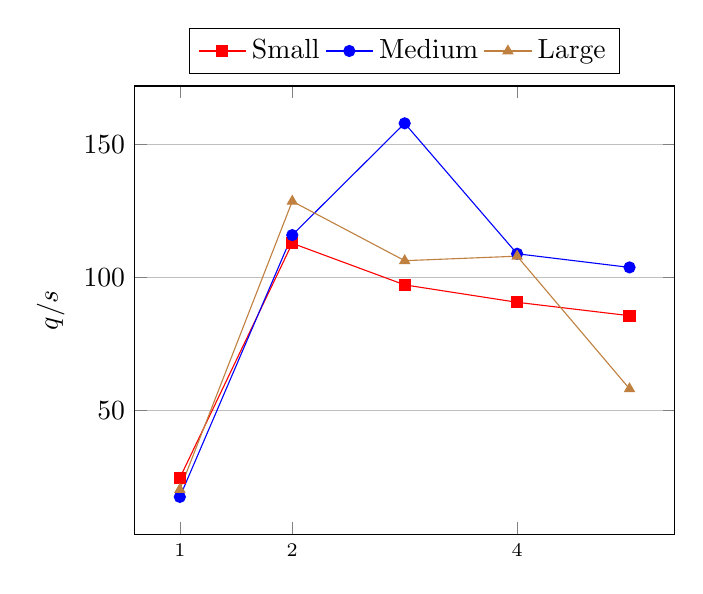
\begin{tikzpicture}
\begin{axis}[
ylabel=$q/s$,
x tick label style={font=\scriptsize},
legend style={at={(0.5,1.13)}, anchor=north, legend columns=-1},
xtick={1,2,4,8},
%ybar,
ymajorgrids=true,
%bar width=5pt,
]

\addplot[red,mark=square*]
coordinates {(1, 24.614) (2, 112.895) (3, 97.257) (4, 90.697) (5, 85.659)};
\addplot[blue,mark=*]
coordinates {(1, 17.492) (2, 115.986) (3, 158.028) (4, 108.956) (5, 103.826)};
\addplot[brown,mark=triangle*]
coordinates {(1, 20.265) (2, 128.696) (3, 106.352) (4, 108.047) (5, 58.153)};

\legend{Small, Medium, Large}

\end{axis}
\end{tikzpicture}%

    }
    \label{fig:medium-query-rate}
  }%
	\caption{The evolution of the average query rate with respect to the size of the star queries over different dataset size.}
	\label{fig:query-rate}
\end{figure}

\section{Discussion}

While AFOR provides better compression ratio than PFOR, AFOR-2 is slower than
PFOR on position file, suggesting that PFOR exception management is slightly
more efficient than the variable frame length approach of AFOR-2 on very
sparse lists. The number of table lookups in AFOR-2 costs more than the
decoding and patching of the exceptions in PFOR.

In general, FOR even if it has more data to read and decompress still provides
the best query execution time. The reason is that our experiments are
performed using warm cache. We therefore ignore the cost of disk IO
accesses and so we can expect a drop of performance for algorithms with a low
compression ratio such as FOR and PFOR compared to AFOR when executing with a
cold cache.

% Compression and decompression performance do not only depend on the
% compression ratio, but also on the execution flow of the algorithm and the
% number of cycles needed to compress or decompress an integer. Therefore,
% CPU-optimised algorithms providing good compression ratio increase the update
% and query throughputs of web search engines. In that context, AFOR seems to be
% a good candidate since it is well balanced in all aspects: it provides very
% good indexing and querying performance and one of the best compression ratio.
% 
% The Simple encoding family is somehow similar to AFOR. At each iteration, S-64
% encodes or decodes a variable number of integers using CPU optimised routines.
% AFOR is however not tied to the machine words, is simpler to implement and
% provides better compression ratio, compression speed and decompression speed.


\chapter{Self-Indexing Benchmarks}{%
In this section we will discuss the performance of SkipBlock compared to Skip
Lists by building structures on real data and performing set operations. First
we present the benchmarking environment used for comparing the self-indexing
structures. Then we compare the results of the SkipBlock structure to the
theoretical ones, before discussing the benefits of the block-based
self-indexing structure against the original Skip List. }%
\label{chap:self-indexing-bench}
\section{Benchmarking Framework}

The benchmarking framework is the same as in
Chapter~\ref{chap:benchmark-cmp}. In this section I present the benchmark
environment used to evaluate the self-indexing structures.

\subsection{Dataset}

For this benchmark we use inverted lists extracted from the Sindice dataset
from Section~\ref{sec:benchmark:framework-cmp}. Those inverted lists only
contains the entity identifiers values, the self-indexing structures being
built upon an ordered list of records, and since only the raw performance of the
self-indexing structure is measured. The other identifiers (e.g., attributes
or values identifiers) are only relevant when computing queries, thus they are
discarded for this benchmark. A small set from each frequency groups, i.e.,
HIGH, Medium and LOW groups generation presented in
Section~\ref{sec:bench-query-FW}, is extracted but keeping the entities
identifiers stream only. A list from the HIGH group will be longer than one
from the LOW group.

\subsection{Benchmark Design}

In order to have a better view of the raw performance of the self-indexing
structures, we perform two set operations, \emph{exclusion} and
\emph{conjunction}. The lists operated on are taken from one of the
three frequency groups of the Sindice dataset. Conjunction operations perform
the intersection of n lists given as operands. Exclusion operations $L_a
\backslash L_b$ exclude all the records from $L_b$ in $L_a$.

This design is based on the querying benchmark's design from the
Section~\ref{sec:bench-query-FW}. In order to process conjunctive queries, the
inverted lists from each term of the query are retrieved and intersected as
explained in Chapter~\ref{chap:IR}. To process the Boolean operator NOT,
the inverted list of the term the operator is affected to is excluded from the
results. At the core of queries processing, set operation are performed on the
retrieved lists. Based on the notation of the Section~\ref{sec:bench-query-FW},
the conjunction set operation of two inverted lists reflects the same
underlying process when computing 2-AND queries.
A measurement of the evaluation consists in the average time to execute a set
operation.

The benchmark records four information:
\begin{enumerate}
  \item the number of bytes read from the self-indexing structure.
  \item the number of documents identifiers skipped.
  \item the average time needed to perform 1 measure.
  \item the total number of search operations done on the structure as defined
  in Section~\ref{sec:cost-based-cmp}, composed of the number of
  synchronization points read plus the number of records scanned.
\end{enumerate}

The design of the SkipBlock benchmark includes two factors:
\begin{description}
\item[Operands] having two levels: HIGH-HIGH and HIGH-LOW. For instance, the
former value means that there are two operands, the HIGH and LOW inverted lists.
\item[Operation] having two levels: exclusion and conjunction.
\end{description}
Each condition of the design, i.e., HIGH-HIGH, Conjunction, possesses 100
distinct measurements.

\subsection{Implementations}

The SkipBlock model possess two implementations based on the interval search
strategies introduced in Section~\ref{sec:search-interval}. However only the S1
and S2 strategies will be discussed in these results due to a lack of time to
evaluate the others.
\begin{itemize}
  \item The baseline \emph{$I_1$} is the original Skip Lists structure with the
  linear search strategy \emph{S1}.
  \item The implementations \emph{$I_2$} and \emph{$I_3$} use respectively the
  strategies \emph{S1} and \emph{S2}. As a remainder, the S2 strategy uses
  block headers as additional synchronization points within an interval.
\end{itemize}

\section{Results}

For these benchmarks, both the self-indexing structures and the inverted list
are compressed with the VByte algorithm.
Before experimenting on the set operations, we evaluated the performance of the
self-indexing structures solely on skipping records. We first review the
evaluation results on the raw performance of the structures, before discussing
the performance with set operations.

\subsection{Advancing on a List}

In this section we evaluate the raw performance of both self-indexing models to
advance on an ordered list. The Table~\ref{tab:skipping-len} reports these
results on a list of $6\times 10^{8}$ records, records that only consist of
entity identifiers.
The first two rows reports the size in MBytes of the self-indexing structures.
A sequence of equally spaced candidates are searched,
i.e., a small skipping length of 16 and a large one of $13\times 10^{4}$
records. For each skipping length, the self-indexing structure are
parameterized with intervals of 32 and 1024, yielding for SkipBlock
respectively two possible configurations ($\vert B \vert =8, \;p=4$) and
($\vert B \vert =64, \;p=16$). 

For a same interval $\vert I \vert$ the SkipBlock structures
performs less search operations, thus saving CPU cycles as the
Table~\ref{tab:cmp-costs} have shown this aspect. However this benefit is
outweighted by the structure's size on small intervals (i.e., $\vert I \vert =
32$), since more data has to be read into memory.
Despite the predicted processing times reported in the
Table~\ref{tab:predicted-times}, the actual processing time for the SkipBlock
structure is not what was expected, i.e., half the time of the original Skip
List's. This can be explained by the compression algorithm, VByte, which is not
suited for compressing blocks.

We can note that for large skip lengths (i.e., 130 000) the SkipBlock
structures are more than 2 times as fast as the original Skip List, on large
intervals. The reason is that for so large intervals the baseline has its
number of levels considerably reduced, which is not the case for SkipBlock
since it adds in-between levels (e.g. Table~\ref{tab:skip-levels}). On top of
these additional levels, $I_3$ allow to reduce the number of search operations
by 10 times in comparison to the baseline.
When performing small skips, $I_2$ and $I_3$ implementations provide better
time than $I_1$ on large interval.

This experiment showed that the SkipBlock model provides important benefits
when jumping over a large number. With small skipping lengths, more data is
read from the SkipBlock as there are additional levels. In the latter case the
benefit of additional skipping levels is outweighted by the increased amount
of read data. We can conclude that in order to get the most benefit from
SkipBlock, configurations with large interval lengths are the most suited.

\begin{table}
\centering
\resizebox{\linewidth}{!}{%
\begin{tabular}{llc@{\hs}lllc@{\hs}lllc@{\hs}lll}
\toprule
 & $\vert I \vert$ & \phantom{a} & \multicolumn{3}{c}{$I_1$}
& \phantom{a} & \multicolumn{3}{c}{$I_2$} & \phantom{a} &
\multicolumn{3}{c}{$I_3$} \\
\cmidrule{4-6} \cmidrule{8-10} \cmidrule{12-14}
& 32 & \phantom{a} & \multicolumn{3}{c}{40.37 MB} & \phantom{a}&
\multicolumn{3}{c}{83.09 MB} & \phantom{a} & \multicolumn{3}{c}{297.57 MB} \\
& 1024 & \phantom{a} & \multicolumn{3}{c}{2.24 MB} & \phantom{a}&
\multicolumn{3}{c}{2.57 MB} & \phantom{a} & \multicolumn{3}{c}{31.6 MB} \\

\midrule
Length & & \phantom{a} & MB & Time & Ops
& \phantom{a} & MB & Time & Ops
& \phantom{a} & MB & Time & Ops \\
\multirow{2}{*}{16} & 32
&\phantom{a}& 38.11 & 12.9
s $\pm$ 135.1 ms & \numprint{338104836} 
&\phantom{a}& 59.72 & 13.8 s $\pm$ 96.8
ms & \numprint{324999973}
&\phantom{a}& 131.25 & 19.3 s $\pm$
132.1 ms & \numprint{212499973} \\
& 1024
&\phantom{a}& 2.24 & 12.6 s $\pm$ 117.7
ms & \numprint{591797454}
&\phantom{a}& 2.46 &
12.0 s $\pm$ 208.6 ms & \numprint{591250005}
&\phantom{a}& 29.28 & 14.0 s $\pm$
88.7 ms & \numprint{459999997} \\
\\
\multirow{2}{*}{\numprint{130000}} & 32
&\phantom{a}& 0.54 &
48.0 ms $\pm$ 5.8 ms & \numprint{211963}
&\phantom{a}& 0.30 & 42.3 ms $\pm$ 8.8 ms
& \numprint{109174}
&\phantom{a}& 0.31 & 47.8 ms $\pm$ 3.1 ms
& \numprint{95326} \\
& 1024
&\phantom{a}& 2.10 & 112.7 ms $\pm$
3.5 ms & \numprint{2883453}
&\phantom{a}& 0.33 & 46.1 ms $\pm$ 2.8 ms
& \numprint{2398582}
&\phantom{a}& 0.44 & 39.5 ms $\pm$ 2.1 ms
& \numprint{283796} \\
\bottomrule
\end{tabular}}
\caption{Self-indexing structures performance with equally spaced (i.e.,
$Length$) candidates. \emph{MB} stands for the number of MBytes read from the
structure. $Ops$ reports the total number of search operations performed
(i.e., the number of synchronization points read plus the number of scanned
records).}
\label{tab:skipping-len}
\end{table}

\subsection{Set Operations Results}
\label{sec:self-indexing-res}

For these benchmarks, both the self-indexing structures and the inverted list
are compressed with the VByte algorithm, so that the differences in
performance between the two structures are not caused by the compression
technique.

The performance of the self-indexing structures is compared based on the time
to perform a set operation, on the number of records that had to be scanned
from the inverted list to search for the candidates, and on the size of the
structure. We can note that the The raw results are reported in the
Table~\ref{tab:conjunction} and Table~\ref{tab:exclusion} in the appendix. For
each operands type (i.e., HIGH:HIGH or HIGH:LOW) and implementations, the best
execution time is taken and reported in the plots of the
Figure~\ref{fig:conj-excl-res}.

We observe from the plots that for either operations on two large lists (i.e.,
HIGH:HIGH type), the SkipBlock configuration of the implementation $I_3$
provides slightly better time than the original while reducing the number of
scanned records by $10^7$. However this has an impact on the structure's size
with an increase of 20 MBytes in comparison to the original model. With set
operations over lists of different sizes (i.e., LOW:HIGH type), we observe the
opposite: by scanning slightly more records and with comparable running times,
the implementation $I_3$ halves the structure's size by at least two.

For set operations on very dense lists, we are able to skip over a large number
of records with the SkipBlock model by increasing the structure's size, while
still providing similar running time as the original model. For set operations
on lists presenting a high size discrepancy, the SkipBlock model is able to
greatly reduce the structure's size while still providing similar running times.

With regards to the raw results of the Appendix~\ref{app:self-indexing:results},
this comforts the conclusion of the previous section that the SkipBlock model
provides more benefits with large intervals. We can note that the implemented
search strategies on intervals are simple ones. Thus it is possible to improve
performances by either changing the strategy, or by using an other compression
method. Indeed we used for this benchmark the VByte algorithm which is not a
block-based algorithm and thus does not profit from all the advantages of the
SkipBlock model. With a compression technique such as AFOR, we are effectively
able to reduce the size of the structure by using the frame skipping technique
(Section~\ref{sec:afor-skip}).

We can conclude that the SkipBlock model provides implementations, on large
interval lengths (e.g., 4096), that trade the structure's size cost over its
searching cost.

\begin{figure}
\centering
\resizebox{\linewidth}{!}{%
\subfloat[Two HIGH operands.] {

\begin{tikzpicture}
\begin{axis}[
        scatter/classes={
		a={mark=o},
		b={mark=star},
		c={mark=square}
% 		d={mark=diamond},
% 		e={mark=triangle}
  },
  xlabel=$Time \; (s)$,
  ylabel=$Scans$,
  mark options={scale=2},
  legend style={font=\scriptsize},
]

\addplot[red,scatter, only marks]
plot[scatter src=explicit symbolic]
coordinates {
% 	(3.400, 55766922) [a]
% 	(2.492, 55882733) [b]
% 	(2.484, 65538236) [c]
% 	(2.541, 73415418) [d]
% 	(2.619, 85376552) [e]

% 	(3.400, 50197056) [a]
% 	(2.492, 52524966) [b]
% 	(2.484, 64766407) [c]
% 	(2.541, 72983836) [d]
% 	(2.619, 85129635) [e]
	
	(2.484, 64766407) [a]
	(2.517, 72893207) [b]
	(2.582, 54730557) [c]
};

\addplot[blue,scatter, only marks]
plot[scatter src=explicit symbolic]
coordinates {
	(16.836, 54212443) [a]
	(15.826, 54205740) [b]
	(15.783, 42438570) [c]
};

% \addplot+[blue,scatter, only marks]
% plot[scatter src=explicit symbolic]
% coordinates {
% % 	(3.631, 53390244) [a]
% % 	(2.650, 54471140) [b]
% % 	(2.844, 65153966) [c]
% % 	(2.517, 73224689) [d]
% % 	(2.925, 85264977) [e]
% 	(3.631, 47270398) [a]
% 	(2.650, 51058497) [b]
% 	(2.844, 64576706) [c]
% 	(2.517, 72893207) [d]
% 	(2.925, 85080396) [e]
% };
% 
% \addplot+[green,scatter, only marks]
% plot[scatter src=explicit symbolic]
% coordinates {
% % 	(3.746, 53680730) [a]
% % 	(3.795, 53203556) [b]
% % 	(2.646, 54160474) [c]
% % 	(2.627, 56475877) [d]
% % 	(2.582, 56514322) [e]
% 	(3.746, 33665878) [a]
% 	(3.795, 42187630) [b]
% 	(2.646, 51063586) [c]
% 	(2.627, 54730109) [d]
% 	(2.582, 54730557) [e]
% };

\legend{$I_1$, $I_2$, $I_3$}
\end{axis}
\end{tikzpicture}

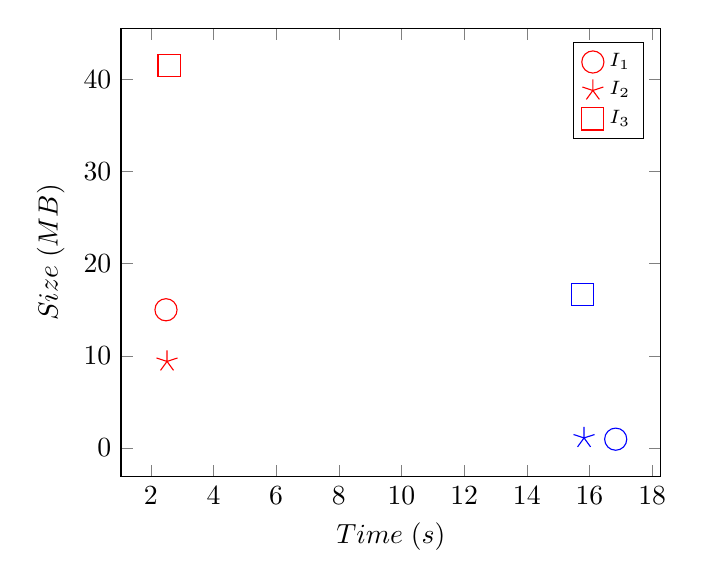
\begin{tikzpicture}
\begin{axis}[
        scatter/classes={
		a={mark=o},
		b={mark=star},
		c={mark=square}
% 		d={mark=diamond},
% 		e={mark=triangle}
  },
  xlabel=$Time \; (s)$,
  ylabel=$Size \; (MB)$,
  mark options={scale=2},
  legend style={font=\scriptsize},
  legend pos= north east
]

\addplot[red,scatter, only marks]
plot[scatter src=explicit symbolic]
coordinates {
% 	(3.400, 12.02) [a]
% 	(2.492, 7.36) [b]
% 	(2.484, 2.97) [c]
% 	(2.541, 1.66) [d]
% 	(2.619, 0.95) [e]
	
	(2.484, 15) [a]
	(2.517, 9.39) [b]
	(2.582, 41.53) [c]
};

\addplot[blue,scatter, only marks]
plot[scatter src=explicit symbolic]
coordinates {
	(16.836, 0.941) [a]
	(15.826, 1.076) [b]
	(15.783, 16.69) [c]
};

% \addplot+[blue,scatter, only marks]
% plot[scatter src=explicit symbolic]
% coordinates {
% 	(3.631, 14.10) [a]
% 	(2.650, 9.16) [b]
% 	(2.844, 2.25) [c]
% 	(2.517, 1.30) [d]
% 	(2.925, 0.74) [e]
% };
% 
% \addplot+[green,scatter, only marks]
% plot[scatter src=explicit symbolic]
% coordinates {
% 	(3.746, 40.83) [a]
% 	(3.795, 23.87) [b]
% 	(2.646, 7.60) [c]
% 	(2.627, 4.99) [d]
% 	(2.582, 4.81) [e]
% };

\legend{$I_1$, $I_2$, $I_3$}
\end{axis}
\end{tikzpicture}


}}\quad
\resizebox{\linewidth}{!}{%
\subfloat[Two operands, one HIGH and one LOW.] {

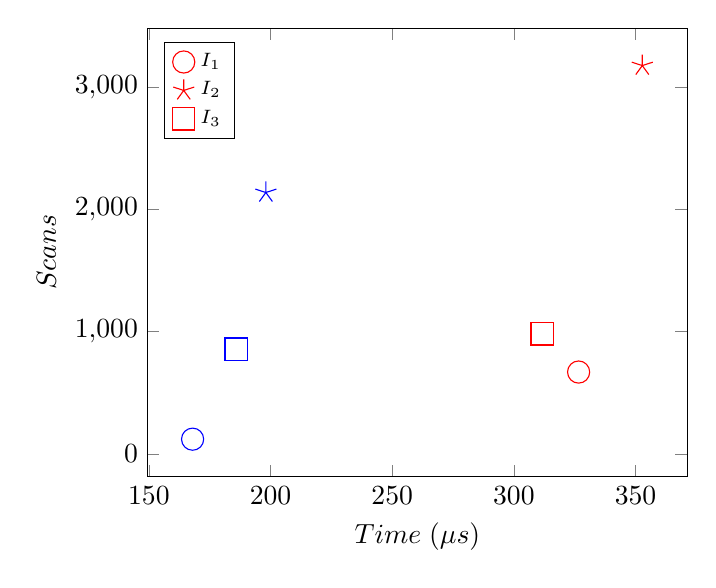
\begin{tikzpicture}
\begin{axis}[
        scatter/classes={
		a={mark=o},
		b={mark=star},
		c={mark=square}
% 		d={mark=diamond},
%  		e={mark=triangle}
  },
  xlabel=$Time \; (\mu s)$,
  ylabel=$Scans$,
  mark options={scale=2},
  legend style={font=\scriptsize},
  legend pos= north west
]

\addplot[red,scatter, only marks]
plot[scatter src=explicit symbolic]
coordinates {
% 	(363.501, 1398) [a]
% 	(326.611, 2088) [b]
% 	(545.605, 9659) [c]
% 	(579.102, 13397) [d]
% 	(735.205, 24296) [e]

% 	(363.501, 447) [a]
% 	(326.611, 670) [b]
% 	(545.605, 4315) [c]
% 	(579.102, 8407) [d]
% 	(735.205, 16207) [e]

	(326.611, 670) [a]
	(352.783, 3176) [b]
	(311.572, 982) [c]
};

\addplot[blue,scatter, only marks]
plot[scatter src=explicit symbolic]
coordinates {
	(167.969, 121) [a]
	(198.083, 2138) [b]
	(185.840, 858) [c]
};

% \addplot+[blue,scatter, only marks]
% plot[scatter src=explicit symbolic]
% coordinates {
% % 	(581.592, 932) [a]
% % 	(521.191, 990) [b]
% % 	(352.783, 3176) [c]
% % 	(432.813, 5718) [d]
% % 	(453.247, 8605) [e]
% 	(581.592, 329) [a]
% 	(521.191, 489) [b]
% 	(352.783, 2733) [c]
% 	(432.813, 5292) [d]
% 	(453.247, 8100) [e]
% };
% 
% \addplot+[green,scatter, only marks]
% plot[scatter src=explicit symbolic]
% coordinates {
% % 	(640.820, 862) [a]
% % 	(585.107, 820) [b]
% % 	(381.714, 1102) [c]
% % 	(370.581, 1539) [d]
% % 	(311.572, 1739) [e]
% 	(640.820, 150) [a]
% 	(585.107, 234) [b]
% 	(381.714, 521) [c]
% 	(370.581, 982) [d]
% 	(311.572, 982) [e]
% };

% \legend{16, 32, 256, 512, 1024}
\legend{$I_1$, $I_2$, $I_3$}
\end{axis}
\end{tikzpicture}

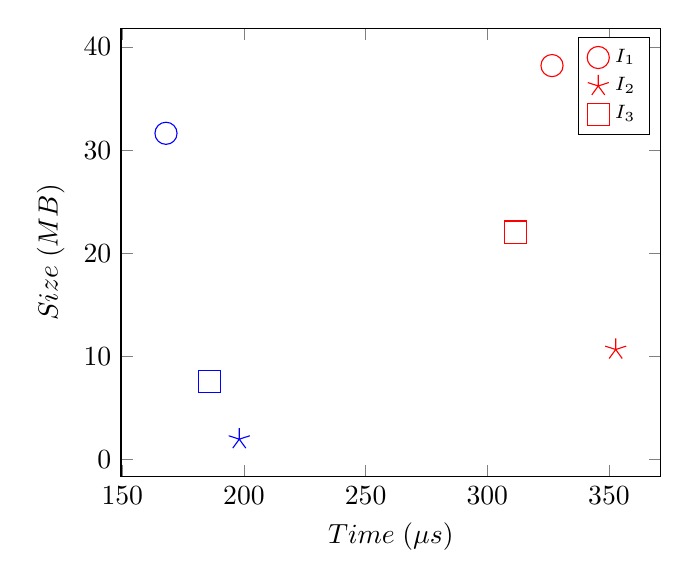
\begin{tikzpicture}
\begin{axis}[
        scatter/classes={
		a={mark=o},
		b={mark=star},
		c={mark=square}
% 		d={mark=diamond},
%  		e={mark=triangle}
  },
  xlabel=$Time \; (\mu s)$,
  ylabel=$Size \; (MB)$,
  mark options={scale=2},
  legend style={font=\scriptsize},
%   legend pos= north west
]

\addplot[red,scatter, only marks]
plot[scatter src=explicit symbolic]
coordinates {
% 	(363.501, 0.004) [a]
% 	(326.611, 0.006) [b]
% 	(545.605, 0.024) [c]
% 	(579.102, 0.022) [d]
% 	(735.205, 0.032) [e]
	
	(326.611, 38.2) [a]
	(352.783, 10.65) [b]
	(311.572, 22.05) [c]
};

\addplot[blue,scatter, only marks]
plot[scatter src=explicit symbolic]
coordinates {	
	(167.969, 31.63) [a]
	(198.083, 1.95) [b]
	(185.840, 7.57) [c]
};

% \addplot+[blue,scatter, only marks]
% plot[scatter src=explicit symbolic]
% coordinates {
% 	(581.592, 0.0031) [a]
% 	(521.191, 0.0026) [b]
% 	(352.783, 0.0023) [c]
% 	(432.813, 0.0023) [d]
% 	(453.247, 0.0027) [e]
% };
% 
% \addplot+[green,scatter, only marks]
% plot[scatter src=explicit symbolic]
% coordinates {
% 	(640.820, 0.0034) [a]
% 	(585.107, 0.0028) [b]
% 	(381.714, 0.0027) [c]
% 	(370.581, 0.0027) [d]
% 	(311.572, 0.0034) [e]
% };

\legend{$I_1$, $I_2$, $I_3$}
\end{axis}
\end{tikzpicture}
}}
\caption{Conjunction (in red) and exclusion (in blue) set operations. The time
on the x axis is the best average time, from the
Appendix~\ref{app:self-indexing:results}, to perform the operation on the
given operands for an implementation.}
\label{fig:conj-excl-res}
\end{figure}
